%Version 3.1 December 2024
% See section 11 of the User Manual for version history
% DSTRA-GNN Extended Version for SN Computer Science Special Issue
% Special Issue: Pervasive digital services for people's well-being, inclusion and sustainable development

%%%%%%%%%%%%%%%%%%%%%%%%%%%%%%%%%%%%%%%%%%%%%%%%%%%%%%%%%%%%%%%%%%%%%%
%%                                                                 %%
%% Please do not use input commands to include other tex files.       %%
%% Submit your LaTeX manuscript as one .tex document.              %%
%%                                                                 %%
%% All additional figures and files should be attached             %%
%% separately and not embedded in the \TeX\ document itself.       %%
%%                                                                 %%
%% NOTE: This file uses \input{} for development convenience.     %%
%% For submission, combine all sections into a single file.       %%
%%%%%%%%%%%%%%%%%%%%%%%%%%%%%%%%%%%%%%%%%%%%%%%%%%%%%%%%%%%%%%%%%%%%%

\documentclass[pdflatex,sn-basic,Numbered]{sn-jnl}% Basic Springer Nature Reference Style with Numbered Citations

%%%% Standard Packages
\usepackage{graphicx}%
\usepackage{multirow}%
\usepackage{amsmath,amssymb,amsfonts}%
\usepackage{amsthm}%
\usepackage{mathrsfs}%
\usepackage{xcolor}%
\usepackage{textcomp}%
\usepackage{manyfoot}%
\usepackage{booktabs}%
\usepackage{url}%
\usepackage{subfig}%
\usepackage{placeins}%
\usepackage{tikz}%
\usetikzlibrary{arrows.meta, positioning, fit, shapes.multipart, calc, backgrounds}
\usepackage{algorithm}%
\usepackage{algpseudocode}%

\raggedbottom

% Configure natbib for numbered citations in square brackets [1], [2], etc.
% (natbib is already loaded by sn-jnl class, so we configure it here)
\setcitestyle{numbers,square}

% Configure hyperref to make citations appear as regular black text (not blue links)
\hypersetup{
    hidelinks,
    colorlinks=false
}

\begin{document}

\title[Accurate ETA Prediction for Urban Mobility and Well-Being]{Accurate ETA Prediction Using Dynamic Route-Aware Graph Neural Networks for Improved Urban Mobility and Well-Being}

\author[1]{\fnm{Guy} \sur{Tordjman}}

\author[2]{\fnm{Nadav} \sur{Voloch}}\email{nadavv@ruppin.ac.il}

\affil[1]{\orgdiv{Department of Mathematics and Computer Science}, \orgname{The Open University}, \orgaddress{\street{University Road 1}, \city{Ra'anana}, \country{Israel}}}

\affil[2]{\orgdiv{Department of Computer Engineering}, \orgname{Ruppin Academic Center}, \orgaddress{\city{Emek Hefer}, \country{Israel}}}


% ===== BEGIN sections/abstract.tex =====
\abstract{\textbf{Purpose:} Estimated Time of Arrival (ETA) prediction underlies route planning, dispatch, and arrival notifications, yet many systems estimate ETA from traffic history without explicit knowledge of a vehicle's planned route. This work examines whether a vehicle-centered dynamic graph with route awareness improves ETA prediction.

\textbf{Methods:} We present DSTRA-GNN (Dynamic Spatio-Temporal Route-Aware GNN), which integrates vehicle-level dynamics and route intent in a Mixture-of-Experts framework. Vehicles are graph nodes, interaction edges model local traffic context, and a GRU-based temporal aggregator processes sequential graph snapshots. We evaluate on SUMO simulation data and Porto-G, a graph representation of the Porto taxi trajectory dataset (ECML-PKDD 2015).

\textbf{Results:} Ablations over six variants show consistent, compounding gains from route awareness and temporal context. On duration-matched Porto-G, MAE drops from 93.3\,s (static graph only) to 68.1\,s (27\% reduction), performing competitively with trajectory-based baselines such as DeepTTE (68.6\,s) and MetaTTE (69.5\,s). On SUMO, MAE drops from 80.1\,s to 54.8\,s (32\% reduction) under the shared protocol range; on the broader p95-filtered SUMO population, the full model remains the strongest evaluated variant and outperforms applicable classical and graph-native baselines at 72.4\,s MAE.

\textbf{Conclusion:} Vehicle-centered dynamic graphs with explicit route state improve ETA prediction across simulated and real-world data, positioning graph-snapshot ETA modeling as a competitive alternative to trajectory-native sequence models.}

% ===== END sections/abstract.tex =====



% ===== BEGIN sections/keywords.tex =====
\keywords{ETA prediction, spatio-temporal graph neural networks, traffic forecasting, mixture of experts, intelligent transportation systems, urban mobility}

% ===== END sections/keywords.tex =====


\maketitle

\begin{figure*}[t]
    \centering
    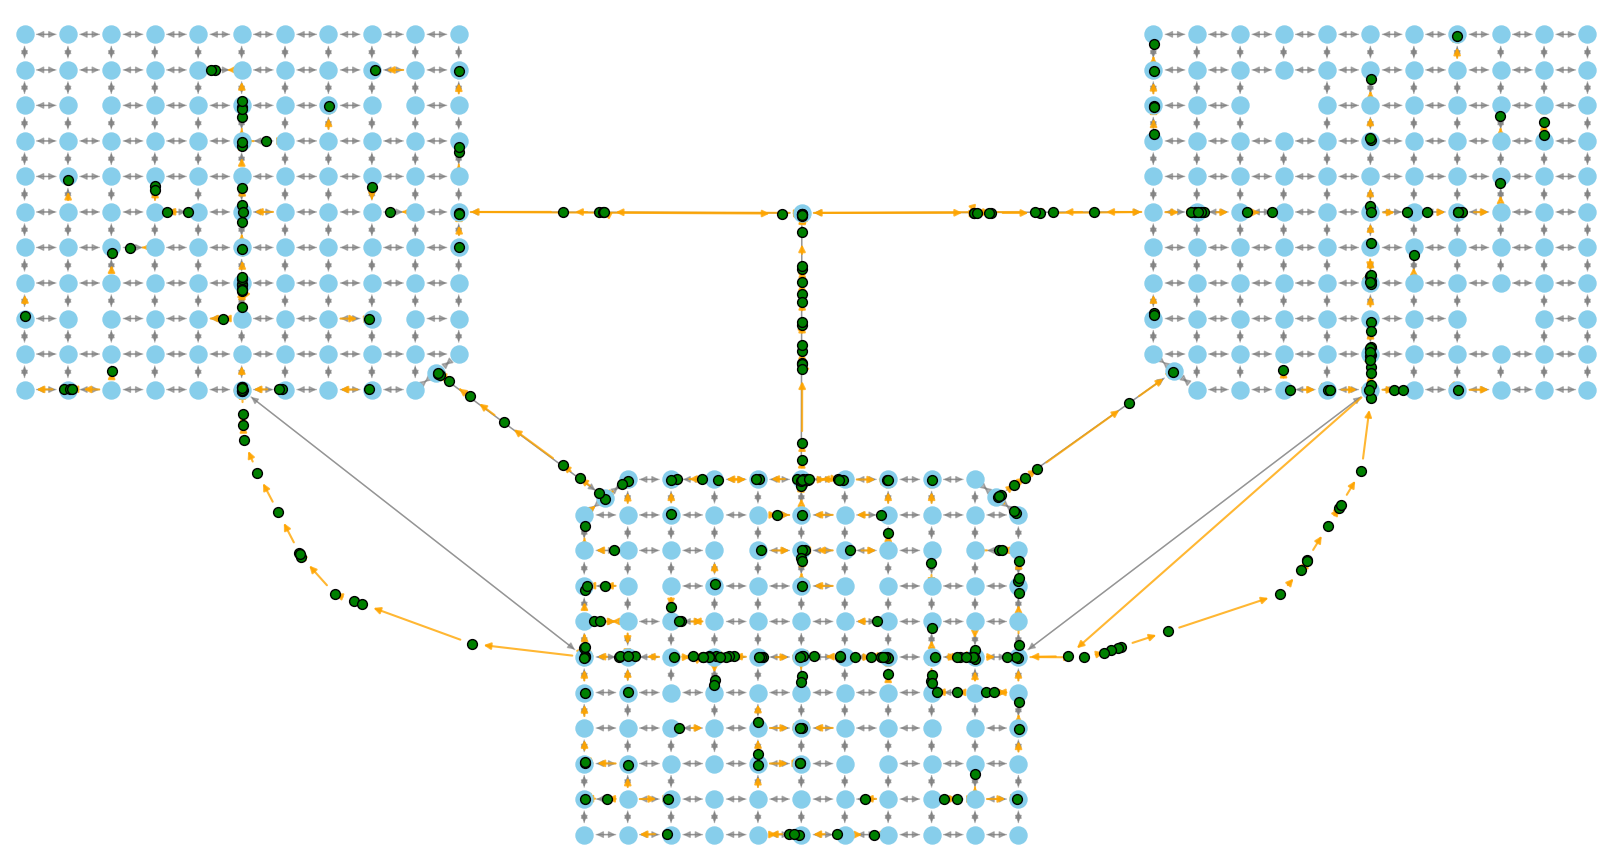
\includegraphics[width=0.80\textwidth]{rush_hour.png}
    \caption{Afternoon rush-hour snapshot spanning the network. Static junction nodes (light blue) and static road edges (gray) form the backbone; dynamic vehicle nodes (green) and dynamic edges (orange arrows) reveal congestion corridors and high-flow funnels.}\label{fig:rush-hour-intro}
\end{figure*}


% ===== BEGIN sections/introduction.tex =====
\section{Introduction}\label{sec1}

Estimated Time of Arrival (ETA) prediction is the task of forecasting how long a trip already underway, or about to begin, will take to complete. Formally, for a vehicle departing at $T_{\mathrm{departure}}$ and predicted to arrive at $T_{\mathrm{arrival}}^{\mathrm{pred}}$,
\begin{equation}
\mathrm{ETA} = T_{\mathrm{arrival}}^{\mathrm{pred}} - T_{\mathrm{departure}}, \label{eq:eta-def}
\end{equation}
i.e., a predicted travel duration rather than a calendar prediction. Despite decades of progress, ETA estimation remains challenging because urban traffic is dynamic and stochastic: congestion builds and dissipates over minutes, and a vehicle's realized travel time depends on conditions not yet observed at departure~\cite{wang2022metatte}.

Accurate ETA matters well beyond convenience. Commuters rely on it to decide when to depart and which route to take, and when an app's estimates prove unreliable, users respond by abandoning its suggested route, padding their departure time as a buffer, or distrusting the app on future trips~\cite{Laor2022,hoseinzadeh2020waze,amin-naseri2018waze}. At the system level, congestion-driven delays cost billions of hours and dollars annually~\cite{INRIX2022Report}, with a proportional cost in excess fuel and emissions~\cite{IEA2022Transport}. Improving ETA accuracy is therefore a lever on daily-life decisions, economic efficiency, and emissions, not only a modeling exercise.

ETA methods have progressed from shortest-path algorithms with static edge costs~\cite{dijkstra1959}, which cannot capture evolving congestion, to models learned directly from historical and real-time data~\cite{chen2016xgboost,deepTTE2018,wang2022metatte}. At production scale, the strongest of these systems already combine road-network graph structure with each vehicle's requested route: Google Maps predicts ETA with a graph neural network over the road network and route~\cite{derrowpinion2021googlemaps}, and Baidu's DuETA likewise encodes route-aware graph context, explicitly modeling how congestion propagates between distant but historically correlated road segments~\cite{dueta2023}. These systems show that dynamic, route-aware graphs work at scale, but both the models and the underlying route data are proprietary, leaving the wider research community unable to train on, evaluate against, or extend them.

Open research, by contrast, has no public dataset, to our knowledge, that combines a road-network graph, per-vehicle dynamics, and explicit route information. Graph-based spatio-temporal models~\cite{dcrnn2018,yu2018stgcn,wu2019graphwavenet} show that a road network is naturally suited to graph learning, since congestion propagates along the same topology the graph encodes -- but they are evaluated on fixed loop-sensor grids~\cite{li2018_metrla,pemsbay}, which record aggregate speed and flow at stationary sensor locations rather than individual vehicles, so no per-vehicle trip or route ever appears in the data. Trajectory-based ETA datasets~\cite{nyc_tlc,moreira2013porto,didi2016,zheng2012geolife} provide per-vehicle trips but not the road graph or each vehicle's pre-planned path, forcing models to infer routes implicitly -- exactly the ambiguity production systems avoid by using their own route data directly.

Simulation offers a way to close this gap: a microscopic traffic simulator such as SUMO~\cite{SUMO2018} can export, by construction, the full road-network graph, per-vehicle dynamics, and each vehicle's ground-truth remaining route at every timestep. Building on our earlier work in traffic simulation and route-aware modeling~\cite{voloch2021,SmartSimulativeRoute2025}, we represent traffic as a dynamic, multi-relational graph in which static junction-to-junction road edges are complemented by time-varying vehicle and interaction edges, as shown in Fig.~\ref{fig:dyn-graph}. Since a simulation-only benchmark cannot by itself show that a representation transfers to real traffic, we additionally convert the Porto taxi trajectory dataset~\cite{moreira2013porto} into the same graph schema, so that the identical model can be evaluated on both a controlled simulation (SUMO) and real-world trips (Porto-G) with no architectural changes between domains.

\textbf{Results.} Across both domains, exposing each vehicle's remaining route and learning temporal context from stable road edges consistently yields the largest accuracy gains over representations that omit them. On duration-matched Porto-G, the full model falls in the same accuracy band as the strongest trajectory-native baselines, with calendar split, duration range, and metrics aligned to the Porto-T evaluation used for DeepTTE and MetaTTE~\cite{deepTTE2018,wang2022metatte}. On the simulated traffic dataset, the same route-aware temporal configuration is the strongest evaluated graph variant under both the shared protocol range and the broader p95-filtered population. These gains hold across a controlled simulation and real-world trips, indicating they are not an artifact of the simulator.

\textbf{Contributions.} First, we propose a dynamic, multi-relational graph representation of traffic that exposes road-network topology, per-vehicle dynamics, and each vehicle's explicit planned route. Second, we define a conversion method that turns a trajectory-based dataset into this graph schema without losing route or timing information, apply it to the publicly released Porto taxi trajectory dataset~\cite{moreira2013porto} to produce Porto-G, and release both Porto-G and a large-scale SUMO simulation dataset publicly on Kaggle~\cite{tordjman2026sumokaggle,tordjman2026portokaggle}. Third, we design DSTRA-GNN with a sparse Mixture-of-Experts head, and show through ablations and retrained Porto and SUMO baselines that graph-snapshot ETA modeling with explicit route state is competitive with strong alternatives.

\textbf{Paper outline.} Sect.~\ref{sec2} reviews related work on ETA estimation and graph-based spatio-temporal models. Sect.~\ref{sec3} introduces the dynamic graph representation, problem formulation, and model architecture. Sect.~\ref{sec4} describes both datasets, the ablation variants, and the external baselines. Sect.~\ref{sec5} presents the ablation and baseline-comparison results. Sect.~\ref{sec6} discusses the findings, and Sect.~\ref{sec7} concludes.

% ===== END sections/introduction.tex =====



% ===== BEGIN sections/related_work.tex =====
\section{Related Work}\label{sec2}

\subsection{Classical pathfinding and routing}
On static graphs $G=(V,E)$ with non-negative edge costs, shortest paths are classically computed via Dijkstra's algorithm~\cite{dijkstra1959}. Alternatives such as Bellman--Ford~\cite{bellman1958routing} and bidirectional search~\cite{pohl1971bi} trade efficiency for generality. More advanced techniques such as A*/ALT landmarks~\cite{goldberg2005}, Contraction Hierarchies~\cite{geisberger2008}, and Customizable Route Planning~\cite{delling2011} scale to web applications but rely on static edge-time models. As a result, they fail to capture evolving congestion or vehicle interactions. Our approach differs fundamentally by learning ETA directly from dynamic traffic graphs rather than static cost assumptions.

\subsection{Trajectory and sensor-based ETA prediction}\label{sec:rw-no-graph}
Many ETA models learn directly from a trip's own recorded data or from fixed sensor measurements, without ever representing the road network as a graph or taking the vehicle's own forward-looking route as a model input.

One group reduces each trip to its raw GPS trace or to a handful of trip-level summary features, a \emph{trajectory representation} of the data. Gradient-boosted trees such as XGBoost~\cite{chen2016xgboost}, applied to handcrafted trip features (distance, time-of-day) on aggregated taxi records (e.g., NYC TLC~\cite{nyc_tlc}, Porto~\cite{moreira2013porto}), give a strong tabular baseline but cannot capture fine-grained spatio-temporal interactions. DeepTTE~\cite{deepTTE2018} instead learns directly from the GPS trace itself, predicting ETA from raw trajectory data on two large-scale taxi datasets: Chengdu (9.7M trajectories, Aug.\ 2014) and Beijing (3.1M trajectories, Apr.\ 2015), with per-trip horizons typically within tens of minutes. MetaTTE~\cite{wang2022metatte} trains a single encoder-decoder model jointly on the Chengdu and Porto taxi trajectory datasets via Reptile-style meta-learning, treating each city as a separate task so the model generalizes to data-sparse cities rather than requiring a dedicated per-city model like DeepTTE. STAD~\cite{abbar2020stad} instead reduces each trip to its origin and destination zone and its departure time, then uses these tabular features to correct the output of a separate, traffic-oblivious routing engine, evaluated on real trip data from Doha, New York City, and Porto.

A second group instead reduces the road network to a \emph{sensor representation}: fixed measurement points or links observed over time, with no individual vehicle or route in the data at all. STANN~\cite{stann2019} applies spatial and temporal attention over an encoder-decoder LSTM to forecast link speeds from sensor data, evaluated on Hong Kong's Traffic Speed Map network (605 links across three regions), a network-wide, long-term forecasting task distinct from per-trip ETA.

Closer to our own setting, our earlier Smart Simulative Route framework~\cite{SmartSimulativeRoute2025} does represent the road network as an explicit graph and does compute a forward-looking route: it anticipates future congestion by enumerating candidate paths and weighting them by the number of vehicles predicted to reach each segment by the time the trip arrives there. However, it remains a classical, heuristic path search over synthetically simulated road networks rather than a model that learns a graph representation from data, so it sits outside the data-driven graph-learning lineage we turn to next.

\subsection{Graph-based, route-agnostic traffic models}\label{sec:rw-graph-no-route}
A third group represents the road network explicitly as a graph, typically with one node per sensor or per road link, so that congestion can propagate along the network's own topology rather than being inferred from trip-level features alone. DCRNN~\cite{dcrnn2018} combines diffusion graph convolutions with recurrent units, predicting future link speeds from sensor data on the METR-LA and PEMS-BAY loop-detector benchmarks at 5--60 min horizons, and became a common backbone for graph-based traffic forecasting. ST-GCN~\cite{yu2018stgcn} replaces the recurrent component with purely convolutional spatio-temporal blocks, predicting speeds from sensor data on PeMSD7, loop-detector data from California's Caltrans Performance Measurement System. Graph WaveNet~\cite{wu2019graphwavenet} further learns an adaptive adjacency matrix rather than relying solely on the physical road graph, evaluated on the same METR-LA and PEMS-BAY sensor benchmarks as DCRNN.

These models inherit the sensor representation of the previous subsection, fixed measurement points observed over time, but add the road network's own topology as an explicit graph. None of them, however, represents an individual vehicle as a graph node or takes a vehicle's own forward route as input, so reported MAEs from this group reflect network-wide speed forecasting rather than per-vehicle arrival time. We reference these methods together with their evaluation scope, city, sensor density, and forecasting horizon, rather than quoting unscoped headline numbers.

\subsection{Graph-based, route-aware production models}\label{sec:rw-graph-route}
A fourth group combines both ingredients above, an explicit road-network graph and the vehicle's own requested route, but only within large-scale, proprietary production systems. Google Maps predicts ETA with a graph neural network over the road network and each driver's requested route~\cite{derrowpinion2021googlemaps}, trained on Google's own live, global traffic data, demonstrating that route-aware graph learning scales to live traffic, though neither the model nor the underlying route data are public. ConSTGAT~\cite{constgat2020} targets per-route ETA in production at Baidu Maps, trained on trip data from Beijing, Shanghai, and Tianjin: it represents the road network as a graph of segments, applies a spatio-temporal graph attention mechanism, and pools local route context with convolutions over the requested route. DuETA~\cite{dueta2023} extends ConSTGAT, also trained on Baidu Maps trip data from Beijing, Shanghai, and Tianjin, by modeling traffic congestion propagation: a congestion-sensitive graph links road segments that are spatially distant but historically correlated in traffic pattern, and a route-aware graph transformer marks which segments lie on the requested route and how far they are from its origin. On these three cities, DuETA reports MAEs of 178.4\,s (Beijing), 155.9\,s (Shanghai), and 171.4\,s (Tianjin), with larger relative gains on long routes ($\geq$3\,km) than short ones in an online A/B test.

Unlike these systems, which represent the road network purely as segments and infer route relevance through structural encodings added to each segment, our method represents vehicles themselves as graph nodes and gives each one its own remaining route as an explicit input feature, alongside dynamic interaction edges and temporal context, within a single unified architecture.

\subsection{Summary and positioning}
Across the models surveyed above, graph representation and route awareness each appear in isolation in open research, drawing on trajectory or sensor data, and only appear together in proprietary, production-scale systems built on undisclosed route data. To our knowledge, no public dataset or model pairs a road-network graph, per-vehicle dynamics, and each vehicle's explicit pre-planned route for ETA prediction. Table~\ref{tab:related_work_comparison} summarizes every system discussed above, grouped by whether it uses a road-network graph, individual vehicle dynamics, and an explicit route, and positions our model against this landscape. Because the MAE/MAPE figures cited throughout this section come from different cities, splits, and label definitions, we treat them as context rather than as a benchmark, and instead retrain a comparable baseline ladder under one shared protocol, defined in Sect.~\ref{sec:baselines}.

\begin{table}[t]
    \centering
    \caption{Positioning relative to every ETA and traffic-forecasting system discussed in Sects.~\ref{sec:rw-no-graph}--\ref{sec:rw-graph-route}. \emph{Route}: the vehicle's own pre-planned path is given as a model input, not inferred post-hoc from a realized trace. \emph{Veh.\ dyn.}: represents individual vehicle state and interactions, not only aggregate sensor/segment-level flow. \emph{Public}: dataset is open/public.}
    \label{tab:related_work_comparison}
    {\footnotesize\setlength{\tabcolsep}{1.5pt}%
    \begin{tabular}{@{}lllccc@{}}
        \toprule
        \textbf{System} & \textbf{Dataset} & \textbf{Input representation} & \textbf{Route} & \textbf{Veh.\ dyn.} & \textbf{Public} \\
        \midrule
        GBM (XGBoost)~\cite{chen2016xgboost}              & NYC TLC, Porto              & Tabular feats.               & $\times$     & $\times$     & \checkmark \\
        DeepTTE~\cite{deepTTE2018}                        & Chengdu, Beijing            & Raw GPS trajectory           & $\times$     & $\times$     & \checkmark \\
        MetaTTE~\cite{wang2022metatte}                    & Chengdu, Porto              & GPS traj.\ (multi-city)      & $\times$     & $\times$     & \checkmark \\
        STAD~\cite{abbar2020stad}                         & Doha, NYC, Porto            & Tabular (zone + time)        & $\times$     & $\times$     & \checkmark$^{*}$ \\
        STANN~\cite{stann2019}                            & Hong Kong               & Sensor-grid series           & $\times$     & $\times$     & $\times$ \\
        Sim.\ Route~\cite{SmartSimulativeRoute2025}       & Synthetic networks          & Road graph (heuristic)       & \checkmark   & $\times$     & $\times$ \\
        DCRNN~\cite{dcrnn2018}                            & METR-LA, PEMS-BAY           & Sensor graph                 & $\times$     & $\times$     & \checkmark \\
        ST-GCN~\cite{yu2018stgcn}                         & PeMSD7                      & Sensor graph                 & $\times$     & $\times$     & \checkmark \\
        Graph WaveNet~\cite{wu2019graphwavenet}           & METR-LA, PEMS-BAY           & Sensor graph (learned adj.)  & $\times$     & $\times$     & \checkmark \\
        Google Maps~\cite{derrowpinion2021googlemaps}     & Google Maps (global)        & Road graph + route           & \checkmark   & $\times$     & $\times$ \\
        ConSTGAT~\cite{constgat2020}                      & Beijing, Shanghai, Tianjin  & Road graph + route           & \checkmark   & $\times$     & $\times$ \\
        DuETA~\cite{dueta2023}                            & Beijing, Shanghai, Tianjin  & Road graph + route           & \checkmark   & $\times$     & $\times$ \\
        \midrule
        \textbf{Ours (DSTRA-GNN)}                         & SUMO, Porto-G               & Per-veh.\ graph + route      & \checkmark   & \checkmark   & \checkmark \\
        \bottomrule
    \end{tabular}}%

    \vspace{4pt}
    {\footnotesize $^{*}$STAD's New York City and Porto trip data are open. Its Doha trip data are proprietary.}
\end{table}

Our contribution is to combine explicit route intent, road-based temporal aggregation, and a sparse MoE head in a single spatio-temporal GNN for ETA, and to evaluate it against retrained baselines across the available representations: graph-native baselines on SUMO and Porto-G, and trajectory-native baselines on the aligned Porto-T trajectory view.

% ===== END sections/related_work.tex =====



% ===== BEGIN sections/methodology.tex =====
\section{Methodology}\label{sec3}

\subsection{Overview}\label{sec:methodology-overview}
This section first introduces the dynamic, multi-relational graph representation that the rest of the paper builds on, then validates that the representation generalizes beyond simulation. A model trained only on simulated traffic cannot demonstrate that its representation transfers to data outside its own generative assumptions, so real-world validation requires a second, independent data source. Among public traffic datasets, only Porto taxi trajectories~\cite{moreira2013porto} combine GPS sampling dense enough for reliable map-matching with the per-vehicle trip resolution that route-awareness requires. Aggregate sensor datasets such as METR-LA and PEMS-BAY record neither individual routes nor vehicle identity. From this single raw source, we build two comparable datasets, detailed over the next two subsections: Porto-T, a filtered trip-level trajectory dataset used to evaluate trajectory-native baselines, and Porto-G, its graph-converted counterpart, following the same graph schema. Alongside these, we use a third, simulation-derived dataset built with SUMO~\cite{SUMO2018}: because the real-world conversion is bottlenecked by one taxi fleet's coverage of one city and by map-matching error, SUMO supplies a larger, denser dynamic-graph corpus with exact ground-truth topology and routes, free of map-matching noise, serving as our primary testbed for model development and ablations. With SUMO and Porto-G sharing one schema, the remainder of this section defines the prediction problem and presents our model, DSTRA-GNN, which fuses the graph representation with temporal and route context through a Mixture-of-Experts head and is trained identically on both datasets to predict per-vehicle ETA.

\subsection{Route-Aware Dynamic Traffic Graph Representation}\label{sec:dynamic-graph}
We represent the transportation system at snapshot time $t$ as a directed multi-relational graph
\begin{equation}
G_t = \big(V_t, E_t, \{A_t^{(\rho)}, W_t^{(\rho)}\}_{\rho\in\mathcal{R}}\big),
\end{equation}
where:
\begin{itemize}
    \item $V_t = V^j \cup V_t^v$ is the set of nodes at time $t$, consisting of
        \begin{itemize}
            \item $V^j$: static junction nodes, representing intersections in the road network,
            \item $V_t^v$: dynamic vehicle nodes, representing vehicles present at time $t$.
        \end{itemize}
    \item $E_t$ is the set of directed edges at time $t$, partitioned by relation type $\rho$.
    \item $\mathcal{R}$ is the set of relation types (road, traversal, interaction).
    \item $A_t^{(\rho)} \in \{0,1\}^{|V_t|\times |V_t|}$ is the binary adjacency matrix for relation $\rho$ at time $t$.
    \item $W_t^{(\rho)} \in \mathbb{R}_{\ge 0}^{|V_t|\times |V_t|}$ is the optional weighted adjacency for relation $\rho$ (e.g., distance-based interaction weights).
\end{itemize}

\begin{figure}[t]
    \centering
    \resizebox{0.95\linewidth}{!}{% inlined from figures/fig_dynamic_graph.tikz
% TikZ: Dynamic, multi-relational traffic graph
% Junction nodes (V^j) vs. vehicle nodes (V^v_t); road / traversal / interaction edges, with legend.
\tikzset{
  junc/.style={draw, fill=black, text=white, rectangle, rounded corners=1pt, minimum size=7mm, font=\bfseries\small, inner sep=0pt},
  veh/.style={draw=green!45!black, fill=green!15, circle, minimum size=5.5mm, thick, inner sep=0pt},
  roadedge/.style={-{Latex[length=2.2mm]}, thick, black},
  travedge/.style={-{Latex[length=2mm]}, thick, dashed, orange!75!black},
  interedge/.style={-{Latex[length=2mm]}, thick, dotted, red!65!black},
  note/.style={font=\footnotesize, align=left}
}

\begin{tikzpicture}[>=Latex]
% --- Junction nodes (static topology) ---
\node[junc] (A) at (0, 3) {A};
\node[junc] (B) at (0, 0) {B};
\node[junc] (C) at (4.6, 1.5) {C};
\node[junc] (D) at (10.4, 1.5) {D};

% --- Vehicle nodes (dynamic) ---
% Segment B--C: single vehicle (its own head and tail)
\node[veh] (v1) at (2.2, 0.25) {};
% Segment C--D: 3-vehicle chain, ordered by position vh (head, k=1) -> vm (k=2) -> vt (tail, k=3)
\node[veh] (vh) at (6.1, 0.35) {};
\node[veh] (vm) at (7.45, 0.35) {};
\node[veh] (vt) at (8.8, 0.35) {};

% --- Road edges: static junction-junction topology ---
\draw[roadedge] (A) -- (C);
\draw[roadedge] (B) -- (C);
\draw[roadedge] (C) -- (D);

% --- Traversal edges: only head/tail vehicle of each segment's chain <-> its junction ---
\draw[travedge] (B) -- (v1);
\draw[travedge] (v1) -- (C);
\draw[travedge] (C) -- (vh);
\draw[travedge] (vt) -- (D);

% --- Interaction edges: chain of consecutive same-segment vehicles, k = chain order ---
\draw[interedge] (vh) -- (vm) node[midway, below, font=\scriptsize] {$\omega(d_{1,2})$};
\draw[interedge] (vm) -- (vt) node[midway, below, font=\scriptsize] {$\omega(d_{2,3})$};

% --- Legend ---
\begin{scope}[yshift=-1.55cm]
  % row 1: node types
  \node[junc, scale=0.75] (lj) at (0,0) {};
  \node[note, anchor=west] at (0.35,0) {Junction node $V^j$};
  \node[veh, scale=0.75] (lv) at (4.3,0) {};
  \node[note, anchor=west] at (4.65,0) {Vehicle node $V_t^v$};

  % row 2: edge types
  \draw[roadedge] (0,-0.65) -- (0.7,-0.65);
  \node[note, anchor=west] at (0.85,-0.65) {Road edge (static)};
  \draw[travedge] (4.3,-0.65) -- (5.0,-0.65);
  \node[note, anchor=west] at (5.15,-0.65) {Traversal edge (junction$\leftrightarrow$vehicle)};
  \draw[interedge] (4.3,-1.2) -- (5.0,-1.2);
  \node[note, anchor=west] at (5.15,-1.2) {Interaction edge (vehicle$\leftrightarrow$vehicle)};
\end{scope}

\end{tikzpicture}
}
    \caption{Dynamic, multi-relational traffic graph at snapshot $t$. Junction nodes $V^j$ (black squares) connect via static road edges (solid). Vehicle nodes $V_t^v$ (green circles) on each segment form a position-ordered chain linked by interaction edges (red dotted, weight $\omega(d_{k,k+1})$). Only the chain's head and tail vehicle attach to a junction, via a traversal edge (orange dashed).}\label{fig:dyn-graph}
\end{figure}

% Compact components figure: encoder, route encoder, router/MoE
\begin{figure}[t]
    \centering
    \subfloat[Graph encoder (last snapshot)]{\resizebox{0.85\columnwidth}{!}{% inlined from figures/fig_encoder.tikz
% TikZ: Graph Encoder (GATv2 with edge features)
\tikzset{blk/.style={draw, rounded corners=2pt, thick, align=center, inner sep=5pt, fill=black!3},
 op/.style={blk, fill=blue!6}, note/.style={font=\footnotesize, align=left}}

\begin{tikzpicture}[>=Latex, node distance=8mm]
% Input features
\node[blk, minimum width=35mm] (nodes) {Node features \\ $h_v \in \mathbb{R}^d$};
\node[blk, below=of nodes, minimum width=35mm] (edges) {Edge features \\ $e_{uv} \in \mathbb{R}^{d_e}$};

% GATv2 layers
\node[op, right=12mm of nodes, minimum width=40mm] (gat1) {GATv2 Layer 1 \\ attention + aggregation};
\node[op, right=12mm of gat1, minimum width=40mm] (gat2) {GATv2 Layer 2 \\ attention + aggregation};

% Output
\node[blk, right=12mm of gat2, minimum width=35mm] (out) {Node embeddings \\ $h_v' \in \mathbb{R}^d$};

% Connections
\draw[->] (nodes) -- (gat1);
\draw[->] (edges) -- (gat1);
\draw[->] (gat1) -- (gat2);
\draw[->] (gat2) -- (out);

% Labels
\node[note, below=2mm of edges] {static graph features};
\node[note, below=2mm of out] {encoded representations};

\end{tikzpicture}
}}\\[2mm]
    \subfloat[Route encoder (vehicle intent)]{\resizebox{0.85\columnwidth}{!}{% inlined from figures/fig_route_encoder.tikz
% TikZ: Route Encoder (vehicle_route_left)
\tikzset{blk/.style={draw, rounded corners=2pt, thick, align=center, inner sep=5pt, fill=black!3},
 op/.style={blk, fill=green!7}, note/.style={font=\footnotesize, align=left}}

\begin{tikzpicture}[>=Latex, node distance=8mm]
\node[blk, minimum width=42mm] (seq) {route\_left: edge IDs [$e_1,\ldots,e_L$]};
\node[op, right=12mm of seq, minimum width=38mm] (emb) {Edge-ID embedding \\ vocab $\approx1294$, dim 64};
\draw[->] (seq) -- (emb);
\node[op, right=12mm of emb, minimum width=30mm] (pool) {Mean pool};
\draw[->] (emb) -- (pool);
\node[blk, right=12mm of pool, minimum width=32mm] (out) {Route vector (64-d)};
\draw[->] (pool) -- (out);
\end{tikzpicture}



}}\\[2mm]
    \subfloat[Router and Mixture-of-Experts]{\resizebox{0.85\columnwidth}{!}{% inlined from figures/fig_router_moe.tikz
% TikZ: Router + MoE (Top-k=2 over 6 experts)
\tikzset{blk/.style={draw, rounded corners=2pt, thick, align=center, inner sep=5pt, fill=black!3},
 moe/.style={blk, fill=orange!12}, op/.style={blk, fill=black!1}, note/.style={font=\footnotesize, align=left}}

\begin{tikzpicture}[>=Latex, node distance=8mm]
% Inputs
\node[blk, minimum width=40mm] (fused) {Fused vehicle vector};
\node[op, right=12mm of fused, minimum width=40mm] (router) {Router softmax (\(\tau\)) \\ Top-$k=2$};
\draw[->] (fused) -- (router);

% Load balancing label (moved above router)
\node[above=2mm of router, font=\footnotesize] {$\lambda_{lb}$ load-balancing; optional KL-to-uniform};

% Experts row (lowered to make room for top arrows)
\matrix (experts) [row sep=0mm, column sep=6mm, right=16mm of router, below=8mm of router] {
  \node[moe, minimum width=20mm] (e0) {E0}; &
  \node[moe, minimum width=20mm] (e1) {E1}; &
  \node[moe, minimum width=20mm] (e2) {E2}; &
  \node[moe, minimum width=20mm] (e3) {E3}; &
  \node[moe, minimum width=20mm] (e4) {E4}; &
  \node[moe, minimum width=20mm] (e5) {E5}; \\
};

% Routing edges (straight from router to each expert)
\foreach \x in {0,1,2,3,4,5} {
  \draw[->] (router.south) -- (e\x.north);
}

% Combine
\node[blk, below=10mm of experts] (combine) {Weighted combine};
\foreach \x in {0,1,2,3,4,5} {\draw[->] (e\x.south) -- ++(0,-4mm) -| (combine.north);}

\node[blk, right=12mm of combine, minimum width=28mm] (eta) {ETA};
\draw[->] (combine) -- (eta);
\end{tikzpicture}



}}
    \caption{Key components: (a) two-layer GATv2 with edge features. (b) route intent via edge-ID embeddings and mean pooling. (c) sparse Top-$k=2$ routing over six experts with load balancing.}\label{fig:components}
\end{figure}

We define three relation types:
\begin{enumerate}
    \item \textbf{Road edges ($\rho=\text{road}$):} For adjacent junctions $(u,v)$ with legal direction $u\!\to\!v$, we add $(u,v)\in E_t^{(\text{road})}$, encoding static road topology.
    \item \textbf{Traversal edges ($\rho=\text{trav}$):} For each occupied segment $(a,b)$, order the vehicles currently on it by position from $a$ to $b$ as $v_{(1)}^t,\dots,v_{(n)}^t$. We add only $(a, v_{(1)}^t)$ and $(v_{(n)}^t, b)$, linking the segment's upstream and downstream junctions to its head and tail vehicle. Interior vehicles $v_{(2)}^t,\dots,v_{(n-1)}^t$ receive no direct junction edge.
    \item \textbf{Interaction edges ($\rho=\text{inter}$):} Consecutive vehicles on the same segment are chained: we add $(v_{(k)}^t, v_{(k+1)}^t)$ for $k=1,\dots,n-1$, weighted by $\omega(d_{k,k+1}(t)) = e^{-d_{k,k+1}(t)/\lambda}$, where $d_{k,k+1}(t)$ is the spacing between consecutive vehicles. A segment with a single vehicle ($n{=}1$) has no interaction edges, and that vehicle is both head and tail.
\end{enumerate}

\subsubsection{Dynamic Edge Construction}
Static road edges (type 1) already exist in the topology and require no construction. For each road segment, we identify the vehicles currently traveling on it and sort them by distance from the segment's source to destination junction. We connect the source junction to the first (nearest) vehicle and the last (farthest) vehicle to the destination junction with traversal edges (type 2), and connect each vehicle to the next vehicle in sorted order with interaction edges (type 3).

\subsubsection{Node and Edge Features}
Each node and edge type is reduced to a compact engineered feature vector for the encoder, listed in Table~\ref{tab:node-edge-features}. SUMO includes a zone one-hot ($n_{\mathrm{zone}}{=}4$). Porto-G has no zone annotations, so it omits it. The complete raw dataset schema, from which these features are engineered, is released with the SUMO~\cite{tordjman2026sumokaggle} and Porto-G~\cite{tordjman2026portokaggle} datasets on Kaggle.

\begin{table}[t]
    \centering
    \caption{Node and edge features used by the graph encoder, with feature-vector dimension per dataset.}\label{tab:node-edge-features}
    \begin{tabular}{@{}lp{6cm}cc@{}}
        \toprule
        \textbf{Type} & \textbf{Features} & \textbf{SUMO} & \textbf{Porto-G} \\
        \midrule
        Junction  & position $(x,y)$, type one-hot (priority / traffic-light / internal), normalized degree, zone one-hot & 10 & 6 \\
        Vehicle   & type one-hot (bus / passenger / truck), speed, acceleration, current \& destination position, trip progress, route length left, time-of-day \& day-of-week (sin/cos), current-edge demand / occupancy / lane count, zone one-hot & 22 & 18 \\
        Road edge & length, speed limit, lane count (static), avg.\ speed, density, demand, occupancy (dynamic) & 7 & 7 \\
        \bottomrule
    \end{tabular}
\end{table}

\subsubsection{Route Intent}
In addition to graph-based relations, each vehicle node carries a feature called \texttt{vehicle\_route\_left}: the ordered sequence of edge IDs remaining along its pre-computed source--destination path, from the vehicle's current edge (exclusive) to its destination. At trip start, we compute a single shortest path over $E^{\mathrm{road}}$ using fixed, pre-traffic edge costs and record its ordered edge-ID list. At snapshot $t$, we locate the vehicle's current edge within this list and take the suffix following it, which shrinks monotonically as the vehicle progresses. The sequence is summarized by the Route Encoder, shown in Fig.~\ref{fig:components}b (edge-ID embedding with mean pooling), and concatenated into the fused vehicle representation. No other route-derived input is used.

\subsection{Dataset Construction and Preparation}\label{sec:porto-conversion}

\subsubsection{Simulated Traffic Dataset Generation}
The SUMO dataset is built from a synthetic road network rather than an imported city map: a layout designed to resemble a real city, combining two dense urban grids, a suburban ring, and a faster connector zone, visible in Fig.~\ref{fig:rush-hour-intro}. It is generated using a friendly desktop tool we developed for this purpose, built around SUMO and TraCI~\cite{SUMO2018,sumo_data_generator}, which makes it straightforward to configure simulation behavior, validate zone and landmark layout, and optionally inject random untracked trips as robustness noise. Although its road network is considerably smaller than Porto-G's, the simulation produces much denser traffic, with far more vehicles active per snapshot, as Table~\ref{tab:dataset-stats} shows.

After generation, we define a p95-filtered SUMO corpus by removing the longest 5\% of SUMO trips by trip-start duration, using the 95th-percentile cutoff of 2{,}587\,s (43.1\,min). This removes a rare simulator tail of very long trips whose durations are disproportionate to their route lengths and would otherwise dominate aggregate error metrics, while retaining about 94.9\% of SUMO vehicles. We report SUMO in two complementary views: the shared $[315,945]$\,s protocol range used for direct comparison with Porto-G, and this broader p95-filtered population used to characterize performance on most retained SUMO trips.

\subsubsection{Porto-T: Baseline Trajectory Dataset}
We construct Porto-T by filtering the raw Porto taxi dataset~\cite{moreira2013porto}, which spans the complete range of trip durations and distances with no filtering applied, through the following rules:
\begin{enumerate}
    \item \textbf{Rule 1 (duration/distance):} total duration in $[315,945]$\,s and total distance in $[1{,}760,7{,}320]$\,m.
    \item \textbf{Rule 2 (minimum points):} at least two GPS points.
    \item \textbf{Rule 3 (positive travel time):} total travel time strictly positive.
    \item \textbf{Rule 4 (plausible GPS jumps):} no inter-point jump implying a speed above 200\,km/h.
\end{enumerate}
Rules 1--3 are adapted from Table III of the MetaTTE Porto protocol~\cite{wang2022metatte}, so that Porto-T supports a direct comparison of performance against MetaTTE's reported baselines. Rule 4 is our own addition, outside that protocol: without it, trips with corrupted or sensor-glitch GPS traces remain in the data with no physically valid path for a model to learn from, so we remove them. Rule 4 alone rejects 12,659 of the 900,963 trips otherwise passing Rules 1--3 (1.4\%). The result, Porto-T, is the trip-level dataset used to evaluate trajectory-native baselines, defined in Sect.~\ref{sec:baselines}. We split it into train/validation/test using the same MetaTTE calendar date ranges used throughout this paper, given in Sect.~\ref{sec:porto-dataset}.

\subsubsection{Trajectory to Routes Conversion}
Converting a Porto-T trajectory into the graph representation begins by matching its raw GPS polyline to a route over the road network. We perform this conversion with the same desktop tool used to generate the SUMO dataset~\cite{sumo_data_generator}. Because the full Porto-G road network is far larger than any single trip's footprint, we limit the match search for a polyline $P=(p_1,\ldots,p_m)$ to a subnetwork rather than the full city graph: we build a bounding box $B$ around $P$ and compute only over $N_{\mathrm{bb}}=(V_{\mathrm{bb}},E_{\mathrm{bb}})$, the subgraph of road edges intersecting $B$ together with their endpoint junctions. A \emph{scoring pass}, applied to every segment of the polyline as described in Algorithm~\ref{alg:route-edge-weights}, assigns every edge in $E_{\mathrm{bb}}$ a coarse tier: edges whose heading differs from the segment heading by more than $\pi/9$ are discarded, and the rest are ranked by a weighted combination of heading gap and distance from the segment's endpoints to the edge. The top-$k$ ranked edges per segment become primary candidates (tier 1), the next $j$ become secondary (tier 10), and edges never selected by any segment keep tier 1000. A \emph{routing pass}, described in Algorithm~\ref{alg:route-astar}, then finds the best matching route by running A* search once from each of the $k$ primary candidate edges of the first segment, with edge cost weighted by tier and the Euclidean distance to the trip's endpoint as the heuristic, stopping as soon as any run reaches a primary candidate of the last segment. The cheapest of these runs is the matched route, and GPS samples are projected onto it to fix each vehicle's position at every snapshot. Fig.~\ref{fig:route-matching} shows the bounding box and the resulting matched route for a sample trip.

\begin{algorithm}[t]
\caption{Edge-weight scoring pass for a GPS polyline}
\label{alg:route-edge-weights}
\begin{algorithmic}[1]
\Require Polyline $P=(p_1,\ldots,p_m)$; bounding-box subnetwork $N_{\mathrm{bb}}=(V_{\mathrm{bb}},E_{\mathrm{bb}})$ with edge headings $\psi_e$; integers $k,j\ge1$; angle threshold $\theta_{\max}=\pi/9$; trade-off $\lambda>0$.
\Ensure Tier $w(e)\in\{1,10,1000\}$ for every $e\in E_{\mathrm{bb}}$ (lower is better).
\State $w(e)\gets 1000$ for all $e\in E_{\mathrm{bb}}$
\For{each segment $s_i=(p_i,p_{i+1})$, $i=1,\ldots,m-1$}
    \State $\phi_i \gets$ heading of $s_i$; \quad $\mathcal{C}\gets\emptyset$
    \For{each edge $e\in E_{\mathrm{bb}}$ with heading gap $\delta_e=|\phi_i-\psi_e|\le\theta_{\max}$}
        \State $r_e \gets \lambda\delta_e + \tfrac{1}{2}\big(d(p_i,e)+d(p_{i+1},e)\big)$; add $e$ to $\mathcal{C}$
    \EndFor
    \State Sort $\mathcal{C}$ by increasing $r_e$; let $\mathrm{Top}_i$ be the first $k$ edges, $\mathrm{Sec}_i$ the next $j$
    \State $w(e)\gets 1$ for $e\in\mathrm{Top}_i$; \quad $w(e)\gets\min(w(e),10)$ for $e\in\mathrm{Sec}_i$
\EndFor
\end{algorithmic}
\end{algorithm}

\begin{algorithm}[t]
\caption{Route extraction by multi-start A$^\ast$}
\label{alg:route-astar}
\begin{algorithmic}[1]
\Require $N_{\mathrm{bb}}$ with tiers $w(e)$; primary sets $\mathrm{Top}_1,\mathrm{Top}_{m-1}$ from Algorithm~\ref{alg:route-edge-weights}; trip endpoint $p_m$.
\Ensure Lowest-cost route among $k$ multi-start runs.
\State Goal set $G \gets \mathrm{Top}_{m-1}$
\For{each start edge $e\in \mathrm{Top}_1$}
    \State Run A$^\ast$ from $e$ with cost $c(e')=w(e')\cdot\mathrm{len}(e')$ and heuristic $h=$ Euclidean distance to $p_m$, stopping as soon as the search reaches $G$
\EndFor
\State \Return the cheapest of the $k$ resulting routes
\end{algorithmic}
\end{algorithm}

\begin{figure*}[t]
    \centering
    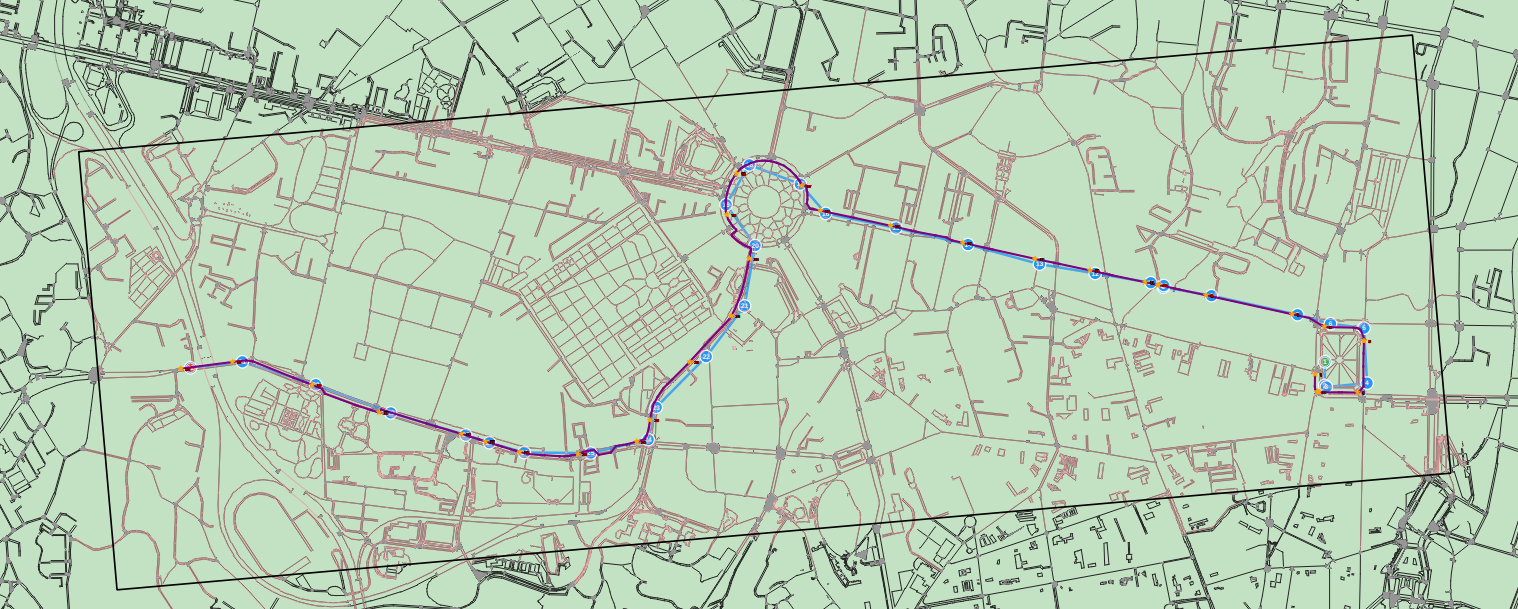
\includegraphics[width=\textwidth]{bb.png}
    \caption{Route matching on the road network. The bounding box, the roads and junctions it restricts the search to (burgundy), the raw GPS polyline (light blue, numbered samples), and the final matched route (dark) are marked, with orange stars showing the GPS points projected onto it.}\label{fig:route-matching}
\end{figure*}

\subsubsection{Porto-G: Graph Dataset Construction and Validation}
Once route matching is applied to every Porto-T trajectory, each matched route is aggregated chronologically into ordered 30-second snapshots, using interpolation to compute each vehicle's current speed and to update the dynamic traffic state on each edge. Conversion succeeds for only around 75\% of trajectories, since a trajectory may fail to map-match onto the road network. A statistical comparison of the converted population against Porto-T's duration distribution showed it skewed toward shorter trips, so we removed this skew with a stratified resampling step that matches the converted population's duration histogram to Porto-T's bucket by bucket, as Fig.~\ref{fig:porto-g-vs-t}a shows. This duration-matched population is the Porto-G dataset used throughout this paper, detailed in Table~\ref{tab:dataset-stats}. The resulting distance distribution still favors shorter trips than Porto-T's even after duration-matching, as Fig.~\ref{fig:porto-g-vs-t}b shows. This reflects \texttt{route\_length} being the road-network shortest path rather than the raw GPS polyline length Porto-T uses. The shift widens Porto-G's distance range rather than narrowing it: the full range of Porto-T's distances remains represented within Porto-G, just with added density toward shorter trips.

\begin{figure}[t]
    \centering
    \subfloat[Trip duration]{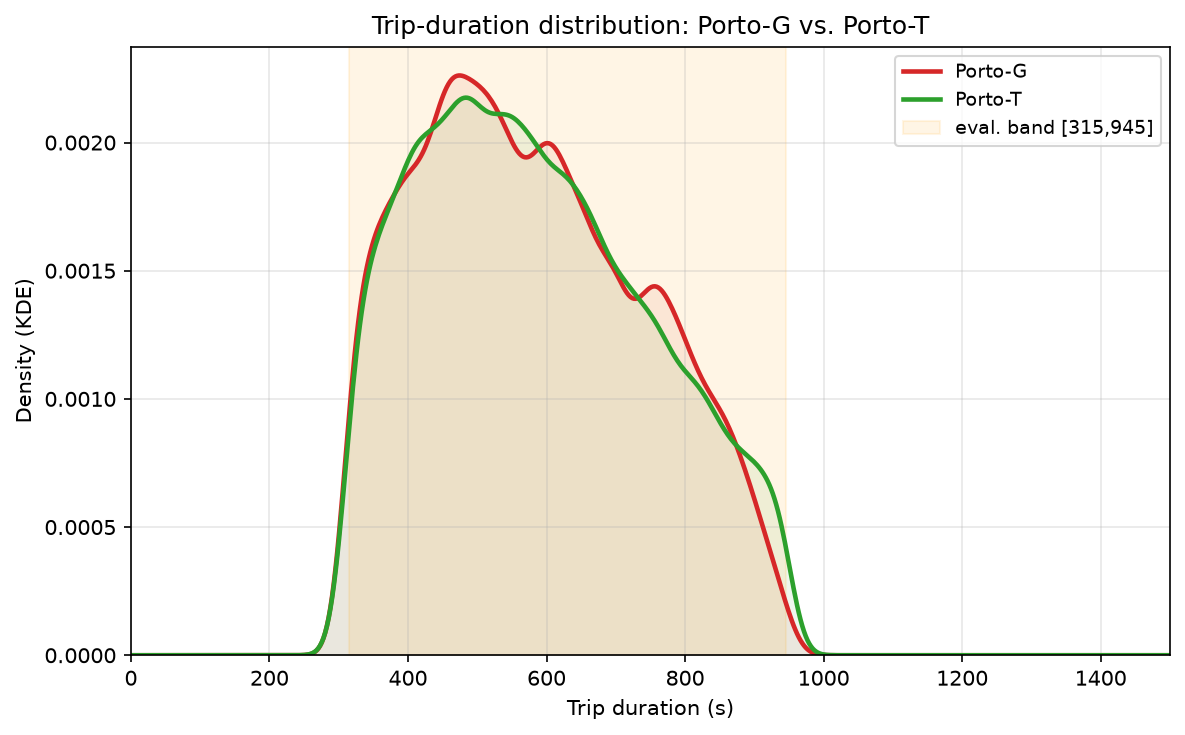
\includegraphics[width=0.48\linewidth]{porto_g_vs_porto_t_duration.png}}\hfill
    \subfloat[Trip distance]{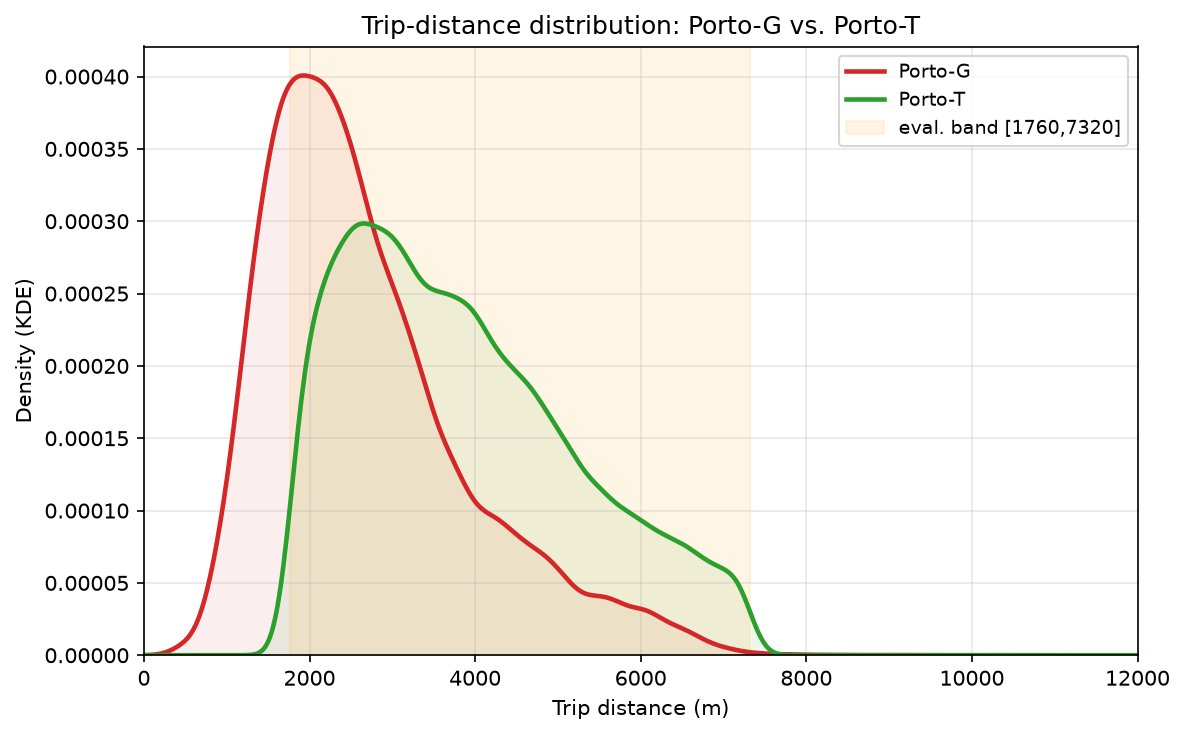
\includegraphics[width=0.48\linewidth]{porto_g_vs_porto_t_distance.png}}
    \caption{Duration-matched Porto-G vs.\ Porto-T density (KDE) for trip duration (a) and distance (b), with the eval band $[315,945]$\,s / $[1{,}760,7{,}320]$\,m shaded. The duration distributions overlap closely within the band by construction, as Table~\ref{tab:dataset-stats} confirms. The distance offset in (b) reflects the shortest-path-route vs.\ GPS-polyline measurement difference, not a sampling artifact.}\label{fig:porto-g-vs-t}
\end{figure}

The resulting dataset, Porto-G, therefore exposes the same $(V_t, E_t, \{A_t^{(\rho)}\}_\rho)$ graph structure, node/edge feature schema, and \texttt{vehicle\_route\_left} convention, so no changes to the model code, training loop, or evaluation metrics are required. The shared schema does not make the data-generating process identical: Porto-G differs from SUMO in route provenance, map-matching noise, and fleet density, and these differences are part of the intended real-world validation. Porto-G inherits Porto-T's chronological train/validation/test assignment after conversion, so every graph snapshot and trip label remains in the same calendar split as its source trajectory.

\subsection{Leakage Considerations}\label{sec:leakage}
This section considers two potential sources of information leakage: (i) whether the edge weights used to compute \texttt{vehicle\_route\_left} via shortest-path search reflect information unavailable at deployment time, and (ii) whether any feature counts future routing demand.

\textbf{Route edge weights.} For both datasets, each vehicle's route is computed once, statically, and independently of current or historical traffic, never as a traffic-conditioned or historical average. For SUMO, the route is computed once per trip using TraCI's Dijkstra implementation~\cite{SUMO2018,dijkstra1959}, weighting each edge by its length divided by its speed limit. For Porto-G, the route is the map-matched path of the vehicle's own recorded GPS trajectory, with no linkage to any other hidden feature.

\textbf{Edge demand.} At each snapshot, the road-edge feature \texttt{edge\_demand} is computed by adding one to an edge's count for every currently active vehicle whose remaining route (\texttt{vehicle\_route\_left}) includes that edge, then normalizing the result. Because it only counts vehicles already present in the current snapshot and their already-fixed remaining plans, it reflects current demand at the time it is observed, not a forecast of future demand, so it does not leak information about routing decisions that have not yet occurred.

\subsection{Temporal Windowing}
ETA prediction requires reasoning over temporal dynamics. We construct a window of $H$ consecutive snapshots:
\begin{equation}
\mathcal{G}_{t-H+1:t} = \{G_\tau\}_{\tau=t-H+1}^t,
\end{equation}
where $H$ is configurable. Consecutive training windows are generated by sliding this window forward through the dataset, with a configurable overlap controlling how many snapshots successive windows share. The prediction target is the ETA of vehicles present in the final snapshot $G_t$.

\subsection{Problem Statement}
Given a temporal window of dynamic graphs $\mathcal{G}_{t-H+1:t}=\{G_{\tau}\}_{\tau=t-H+1}^{t}$, where each snapshot $G_{\tau}$ contains static junction nodes $V^{j}$, dynamic vehicle nodes $V^{v}_{\tau}$, static road edges, and time-varying interaction edges, the goal is to predict per-vehicle ETAs at the final snapshot $t^*{=}t$. Let $\mathcal{V}_t = V^{v}_{t}$ denote vehicles present at time $t$. We learn a function $f_{\theta}$ that maps
\begin{equation}
f_{\theta}\big(\mathcal{G}_{t-H+1:t},\;\texttt{route\_left}_t\big) \;\to\; \hat{\mathbf{y}}_t \in \mathbb{R}^{|\mathcal{V}_t|},
\end{equation}
where $\texttt{route\_left}_t$ is each vehicle's remaining route as of the final snapshot $t$ only, and $\hat{\mathbf{y}}_t[i]$ is the ETA for vehicle $i\in\mathcal{V}_t$. Training minimizes mean absolute error (MAE) over vehicles present at $t$:
\begin{equation}
\mathcal{L}_{\text{MAE}} = \frac{1}{|\mathcal{V}_t|}\sum_{i\in\mathcal{V}_t} \big| \hat{y}_t[i] - y_t[i] \big|.
\end{equation}

\subsection{Model Architecture}
Our DSTRA-GNN model integrates spatial, temporal, and route information. See the complete architecture in Fig.~\ref{fig:temporal-moe-eta}. The main components are:

\begin{itemize}
    \item \textbf{Graph Encoder:} Each snapshot $G_t$ is processed by a 2-layer GATv2-based encoder with edge features, hidden size 128, 4 heads per layer, GELU activations, and LayerNorm residual connections (dropout 0.1), producing embeddings for junction and vehicle nodes, shown in the encoder panel in Fig.~\ref{fig:components}.
    \item \textbf{Temporal Aggregator:} For each pre-final snapshot $\tau\in\{t{-}H{+}1,\ldots,t{-}1\}$ we take the static road-edge features (edge\_type$=0$) and build edge-wise sequences across time. A single-layer GRU (hidden size 128) processes these $H{-}1$ step sequences per edge. The final hidden state for each edge is projected and mean-pooled over all static edges to a graph-level context vector, detailed in Fig.~\ref{fig:gru-detail}. This context is broadcast to all vehicles at $t^*$ for prediction. For \emph{all} temporal variants, temporal context is computed from static road edges only for $t{-}H{+}1\ldots t{-}1$, while the final snapshot $G_t$ is encoded with the appropriate spatial topology (static or full dynamic) per variant. We summarize road edges, which are persistent across the window, rather than vehicles or interaction edges, which are transient, and broadcast one pooled vector to every vehicle rather than conditioning per-route, since ETA depends on network-wide conditions beyond a vehicle's own path.
    \item \textbf{Vehicle Selection:} From the final snapshot $G_t$, we retain only vehicle node embeddings, as these are the prediction targets for ETA.
    \item \textbf{Route Encoder:} Each vehicle's remaining route (\texttt{vehicle\_route\_left}) is embedded via an edge-ID lookup with embedding dimension 64, followed by mean pooling over the variable-length sequence, shown in the route panel in Fig.~\ref{fig:components}b. The pooled route vector is concatenated with the vehicle embedding and temporal context when route awareness is enabled.
    \item \textbf{Fusion and MoE Head:} Vehicle embeddings, enriched with route and temporal context, are fused through an MLP (256 hidden, GELU, LayerNorm, dropout 0.1) into a 192-dim representation and routed to a sparse Top-$k$ Mixture-of-Experts (MoE) head (dropout 0.1), shown in the router panel in Fig.~\ref{fig:components}, where specialized experts capture heterogeneous traffic regimes. We route to $k{=}2$ of 6 experts as a single shared default across datasets: in Table~\ref{tab:moe-expert-sweep}, this setting gives the best SUMO result by a larger margin while remaining within 0.19\,s MAE of the best Porto-G setting, avoiding per-dataset expert-count tuning while keeping the router tractable at our batch size. The output is the ETA prediction for each vehicle.
\end{itemize}

\begin{table}[t]
    \centering
    \caption{Mixture-of-Experts count sensitivity, eval-range MAE (s) at full convergence. \textbf{Bold} = best per column.}\label{tab:moe-expert-sweep}
    \begin{tabular}{@{}lcc@{}}
        \toprule
        \textbf{Experts} & Porto-G & SUMO \\
        \midrule
        2           & 71.22          & 75.37          \\
        \textbf{3}  & \textbf{68.22} & 73.53          \\
        4           & 69.35          & 74.89          \\
        5           & 69.78          & 73.98          \\
        6 (default) & 68.41          & \textbf{72.44} \\
        7           & 70.02          & 75.77          \\
        8           & 72.54          & 76.89          \\
        \bottomrule
    \end{tabular}
\end{table}

% ===== TikZ Diagram of Model Architecture =====
\begin{figure*}[t]
    \centering
    \resizebox{0.88\textwidth}{!}{% inlined from figures/fig_temporal_moe_eta.tikz
% TikZ diagram: DSTRA-GNN (Temporal MoE ETA)
% This file is included by sections/methodology.tex

% Styles used by nodes in this diagram
\tikzset{
  block/.style = {draw, rounded corners=2pt, thick, align=center, inner sep=6pt, fill=black!3},
  small/.style = {draw, rounded corners=2pt, align=center, inner sep=4pt, fill=black!3},
  op/.style    = {block, fill=blue!6},
  opt/.style   = {block, fill=green!7},
  moe/.style   = {block, fill=orange!12}
}

\begin{tikzpicture}[>=Latex, node distance=12mm]

% --- LANE 1: H-1 snapshots (road edge features) ---
\node[block, minimum width=42mm, minimum height=16mm] (snapdeck)
  {$t{-}H{+}1,\ldots,t{-}1$ \\ \footnotesize Road edge features per snapshot};

% faint background cards behind the main one (deck effect)
\begin{scope}[on background layer]
  % soft shadow under/behind the top card (horizontal alignment)
  \node[fill=black!12, draw=none, rounded corners=2pt, minimum width=42mm, minimum height=18mm]
    at ($(snapdeck.center)+(1.2mm,0mm)$) {};
  % aligned background cards with thicker frames (exact same size as snapdeck)
  % use snapdeck's corners to draw identically sized rectangles behind it
  \draw[rounded corners=2pt, line width=1.4pt, draw=black!70, fill=white]
    ($(snapdeck.south west)+(6mm,6mm)$) rectangle ($(snapdeck.north east)+(6mm,6mm)$);
  \draw[rounded corners=2pt, line width=1.4pt, draw=black!70, fill=white]
    ($(snapdeck.south west)+(5mm,5mm)$) rectangle ($(snapdeck.north east)+(5mm,5mm)$);
  \draw[rounded corners=2pt, line width=1.4pt, draw=black!70, fill=white]
    ($(snapdeck.south west)+(4mm,4mm)$) rectangle ($(snapdeck.north east)+(4mm,4mm)$);
  \draw[rounded corners=2pt, line width=1.4pt, draw=black!70, fill=white]
    ($(snapdeck.south west)+(3mm,3mm)$) rectangle ($(snapdeck.north east)+(3mm,3mm)$);
  \draw[rounded corners=2pt, line width=1.4pt, draw=black!70, fill=white]
    ($(snapdeck.south west)+(2mm,2mm)$) rectangle ($(snapdeck.north east)+(2mm,2mm)$);
  \draw[rounded corners=2pt, line width=1.4pt, draw=black!70, fill=white]
    ($(snapdeck.south west)+(1mm,1mm)$)  rectangle ($(snapdeck.north east)+(1mm,1mm)$);
\end{scope}

% --- Temporal module (lane 1) ---
\node[op, below=15mm of snapdeck, minimum width=70mm] (temp)
  {Temporal module: GRU \\ \footnotesize edge-level dynamic road features };

% --- LANE 2: last snapshot -> encoder -> vehicles ---
\node[block, right=38mm of snapdeck, minimum width=42mm, minimum height=12mm] (lastsnap)
  {Last snapshot $t$ \\ \footnotesize Dynamic graph};
\node[op, below=of lastsnap, minimum width=45mm] (encoder)
  {Graph Encoder};
\node[small, below=of encoder] (vehsel) {Select vehicles at $t$};

% --- Route encoder (optional, Full) ---
\node[opt, right=22mm of vehsel, align=left, minimum width=55mm] (routeenc)
  {Route Encoder\\ \footnotesize edge-id embedding + mean pooling\\
   \footnotesize input: $vehicle\_route\_left$ (remaining edge-ID sequence)};

% --- Fusion / Router / Experts / Output ---
\node[op,   below=of vehsel,  minimum width=70mm] (fusion)  {Fusion MLP};
\node[moe,  below=of fusion,  minimum width=70mm] (router)  {Router (softmax, temperature, noise) \\ Top-$k$ selection};

% Six experts laid out horizontally
% Experts arranged in a centered single row (0..5 left to right)
\matrix (expertsrow) [row sep=0mm, column sep=6mm, below=12mm of router] {
  \node[moe, minimum width=24mm] (exp0) {Expert 0}; &
  \node[moe, minimum width=24mm] (exp1) {Expert 1}; &
  \node[moe, minimum width=24mm] (exp2) {Expert 2}; &
  \node[moe, minimum width=24mm] (exp3) {Expert 3}; &
  \node[moe, minimum width=24mm] (exp4) {Expert 4}; &
  \node[moe, minimum width=24mm] (exp5) {Expert 5}; \\
};

\node[block, below=18mm of expertsrow, minimum width=70mm] (pred) {Per-vehicle ETA};

% --- Connections ---
% Lane 1 (temporal): window -> GRU -> fusion (context)
\draw[->] (snapdeck) -- (temp);
\draw[->] (temp.south) |- (fusion.west);

% Lane 2 (spatial): last snapshot -> encoder -> vehicles -> fusion
\draw[->] (lastsnap) -- (encoder);
\draw[->] (encoder) -- (vehsel);
\draw[->] (vehsel) -- (fusion);
\draw[->] (fusion) -- (router);
% router to each expert
\draw[->] (router.south) to[out=-90,in=90] (exp0.north);
\draw[->] (router.south) to[out=-90,in=90] (exp1.north);
\draw[->] (router.south) to[out=-90,in=90] (exp2.north);
\draw[->] (router.south) to[out=-90,in=90] (exp3.north);
\draw[->] (router.south) to[out=-90,in=90] (exp4.north);
\draw[->] (router.south) to[out=-90,in=90] (exp5.north);

% experts to prediction (merged conceptually)
\draw[->] (exp0.south)  |- (pred.west);
\draw[->] (exp1.south)  |- (pred.west);
\draw[->] (exp2.south)  -- (pred.north);
\draw[->] (exp3.south)  -- (pred.north);
\draw[->] (exp4.south)  |- (pred.east);
\draw[->] (exp5.south)  |- (pred.east);

% optional route path (Full)
\draw[->, dashed] (vehsel) -- (routeenc);
\draw[->, dashed] (routeenc.south) |- (fusion.east);

% small notes (optional)
% \node[above=0mm of snapdeck, font=\footnotesize] {Input from sliding window dataset};
% \node[right=2mm of pred,  font=\footnotesize, align=left] {target inverted to seconds for metrics};

\end{tikzpicture}
}
    \caption{DSTRA-GNN architecture. A window of $H{=}30$ dynamic graph snapshots (shown as an overlapped deck) is processed by a \emph{shared} Graph Encoder, with prediction made at the last snapshot $t^*$. In the Full variant, a Route Encoder summarizes each vehicle's remaining path before Fusion and a Top-$k$ MoE head produces per-vehicle ETA.}\label{fig:temporal-moe-eta}
\end{figure*}

\begin{figure}[t]
    \centering
    \resizebox{\linewidth}{!}{% inlined from figures/fig_temporal_gru_detail.tikz
% TikZ: Temporal GRU detail (edge-level sequences)
\tikzset{blk/.style={draw, rounded corners=2pt, thick, align=center, inner sep=4pt, fill=black!3},
 mod/.style={blk, fill=blue!6}, note/.style={font=\footnotesize, align=left}}

\begin{tikzpicture}[>=Latex, node distance=6mm]
% Input sequences per static edge
\node[blk, minimum width=30mm] (e1) {$x_{e_1}^{0..H-2}$};
\node[blk, below=of e1, minimum width=30mm] (e2) {$x_{e_2}^{0..H-2}$};
\node[blk, below=of e2, minimum width=30mm] (e3) {$x_{e_3}^{0..H-2}$};
\node[note, right=2mm of e1] {edge features over time};

% Input projection
\node[mod, right=18mm of e2, minimum width=36mm] (proj) {Input projection};
\draw[->] (e1) -- (proj);
\draw[->] (e2) -- (proj);
\draw[->] (e3) -- (proj);

% GRU cell
\node[mod, right=18mm of proj, minimum width=40mm] (gru) {GRU \newline (hidden $d{=}128$)};
\draw[->] (proj) -- (gru);

% Take final hidden state
\node[mod, right=18mm of gru, minimum width=40mm] (last) {Final hidden state \newline + LayerNorm};
\node[mod, below=of last, minimum width=40mm] (outp) {Output proj (to edge dim)};
\draw[->] (gru) -- (last);
\draw[->] (last) -- (outp);

% Edge-context pooling
\node[blk, right=18mm of outp, minimum width=36mm] (pool) {Mean over edges \newline Graph context};
\draw[->] (outp) -- (pool);

\end{tikzpicture}
}
    \caption{Temporal GRU detail: per-edge feature sequences across $H{-}1$ snapshots are projected, processed by a GRU (hidden size 128), reduced via the final hidden state + LayerNorm, projected back to edge dimension, then mean-pooled over static edges to a graph-level context vector.}\label{fig:gru-detail}
\end{figure}

\subsection{Loss Functions and Training Protocol}\label{sec:loss}
We train the model with supervised regression on ETA targets, in a normalized target space:
\begin{equation}
y_{log} = \log\big(1 + y_{sec}\big)
\end{equation}
\begin{equation}
y_{log,z} = \frac{y_{log} - \mu}{\sigma}
\end{equation}
where $y_{sec}$ is the raw ETA in seconds and $(\mu,\sigma)$ are computed on the training set. The primary loss is MAE computed in this $y_{\log,z}$ space:
\begin{equation}
\mathcal{L}_{\text{MAE}} = \frac{1}{N}\sum_{i=1}^N \big| \hat{y}_i - y_i \big|,
\end{equation}
where $\hat{y}_i$ and $y_i$ are the predicted and true values in $y_{\log,z}$ space. Metrics (MAE, RMSE, MAPE) are reported after inverting to seconds. The optimization objective includes MoE load balancing and optional router regularization:
\begin{equation}
\mathcal{L} = \mathcal{L}_{\text{MAE}} + \lambda_{\text{lb}}\,\mathcal{L}_{\text{lb}} \;\; (\text{and optionally }
\lambda_{\text{kl}}\,\mathrm{KL}(p\,\Vert\,\text{Uniform})),
\end{equation}
where $\mathcal{L}_{\text{lb}}$ encourages uniform expert usage via importance/load terms from the router, and $p$ are routing probabilities. We set $\lambda_{\text{lb}}{=}0.05$, an optional $\lambda_{\text{kl}}{=}0.002$, a router temperature of 1.2, and additive Gaussian logit noise (std 0.15) during training.

We train with AdamW (lr $10^{-3}$, weight decay $10^{-2}$), linear warmup then cosine annealing ($T_{\text{max}}{=}200$), batch size 2, 200 epochs. This configuration is shared by all six ablation variants on both SUMO and Porto-G, with no per-dataset or per-variant tuning, isolating the effect of the architectural toggles, defined in Sect.~\ref{sec:ablation-variants}, rather than per-run tuning. Training runs on a single NVIDIA RTX 5080 GPU at batch size 2: one step takes $\sim$0.18\,s on SUMO ($1{,}294$ road edges, up to $\sim$282 active vehicles per snapshot) and a comparable time on Porto-G (larger but sparser graphs, $\sim$10--15 active vehicles per snapshot), with a full run completing within a few hours per seed per variant and no training instability observed.

For completeness, we report the following definitions used in evaluation:
\begin{equation}
\mathrm{RMSE} = \sqrt{\frac{1}{N}\sum_{i=1}^{N} (\hat{y}_i - y_i)^2}
\end{equation}
\begin{equation}
\mathrm{MAPE}(\%) = 100\cdot \frac{1}{N}\sum_{i=1}^{N} \left|\frac{\hat{y}_i - y_i}{y_i}\right|
\end{equation}
All metrics are computed in seconds. The precise evaluation protocol and population, including trip-start protocol-range metrics and retained-row SUMO p95 metrics, are defined in Sect.~\ref{sec4}.

\paragraph{Complexity and inference.}
Per-snapshot spatial encoding is $\mathcal{O}(|E_t|)$. Temporal aggregation is $\mathcal{O}(|E_\text{road}|\cdot(H{-}1))$ over static road edges only (GRU processes each edge sequence sequentially). Inference processes a window and emits per-vehicle ETAs at $t^*$ with negligible overhead beyond a single forward pass of the encoder plus GRU temporal aggregator: on a single RTX 5080, the full Porto-G test split runs at $\sim$58 windows/s ($\approx$17\,ms/window, batch size 1, including data loading), well within the real-time budget for the 30\,s snapshot cadence used throughout this work.


% ===== END sections/methodology.tex =====



% ===== BEGIN sections/experiments.tex =====
\section{Experimental Evaluation}\label{sec4}

\subsection{Datasets}\label{sec:porto-dataset}
We evaluate on the three datasets defined in Sect.~\ref{sec:porto-conversion}: SUMO and Porto-G for graph-based models, and Porto-T for trajectory-native baselines.

All three datasets use chronological train/validation/test splits with no overlap. SUMO is split into two weeks for training, followed by one week for validation and one week for testing. Porto-T and Porto-G use the shared calendar split train: 2013-07-01--2014-02-28, validation: 2014-03-01--2014-04-01, and test: 2014-05-01--2014-07-01. Table~\ref{tab:dataset-stats} summarizes the split sizes, scale, and trip statistics used in evaluation. Topology and snapshot counts apply only to the graph datasets, so they are omitted for Porto-T.

\begin{table}[t]
    \centering
    \caption{Dataset topology, scale, and trip statistics (all splits combined). Porto-G figures reflect the duration-matched population used throughout this paper, as described in Sect.~\ref{sec:porto-conversion}. Road edges also give the Route Encoder's vocabulary size.}\label{tab:dataset-stats}
    {\footnotesize\setlength{\tabcolsep}{4pt}%
    \begin{tabular}{@{}lccc@{}}
        \toprule
         & \textbf{SUMO} & \textbf{Porto-G} & \textbf{Porto-T} \\
        \midrule
        Junctions                       & 362     & 75{,}264 & -- \\
        Road edges                      & 1{,}294 & 79{,}160 & -- \\
        Network length (km)             & 676     & 4{,}945  & -- \\
        Sampling period (s)             & 30      & 30       & 15 \\
        Snapshots (train/val/test)      & 40{,}312 / 20{,}160 / 20{,}221 & 682{,}968 / 89{,}936 / 172{,}560 & -- \\
        Window overlap (snapshots)      & 10      & 10       & -- \\
        Trips (total)                   & 798{,}919 & 420{,}958 & 819{,}517 \\
        Avg.\ active vehicles/snapshot  & 287.8   & 8.1 & -- \\
        Trip duration mean / median (s) & 856 / 851       & 580 / 570       & 584 / 570 \\
        Trip duration std (s)           & 432             & 161             & 164 \\
        Trip distance mean / median (m) & 11{,}253 / 12{,}107 & 2{,}698 / 2{,}421 & 3{,}851 / 3{,}634 \\
        Mean vehicle speed (m/s)        & 13.87               & 6.53            & 6.77 \\
        Protocol-range fraction         & 0.52                & 1.00            & 1.00 \\
        \bottomrule
    \end{tabular}}%
\end{table}

\begin{figure}[!htbp]
    \centering
    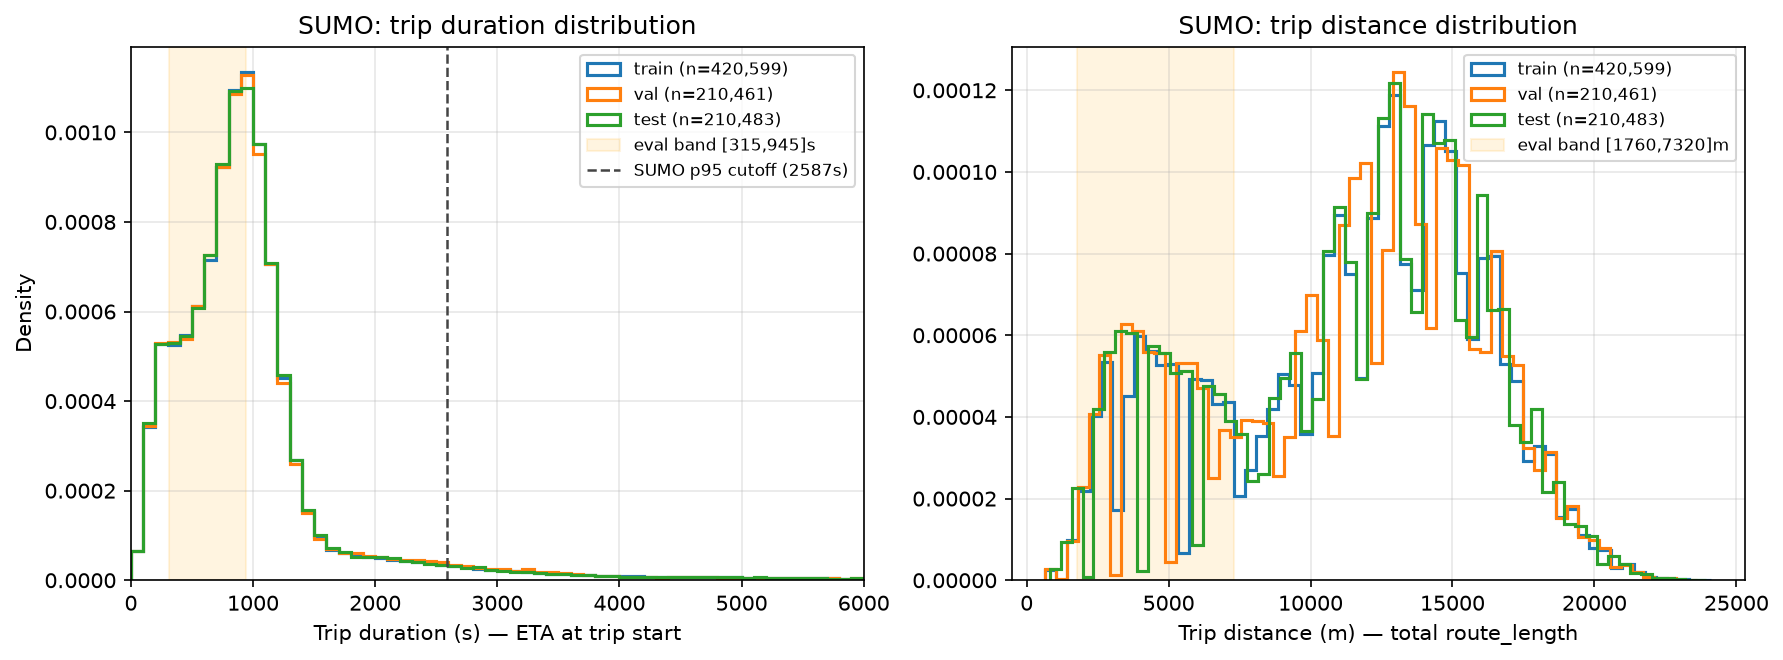
\includegraphics[width=0.95\linewidth]{sumo_trip_duration_distance_distributions.png}
    \caption{SUMO trip duration and distance distributions by chronological split.}\label{fig:sumo-trip-dist}
\end{figure}

\begin{figure}[!htbp]
    \centering
    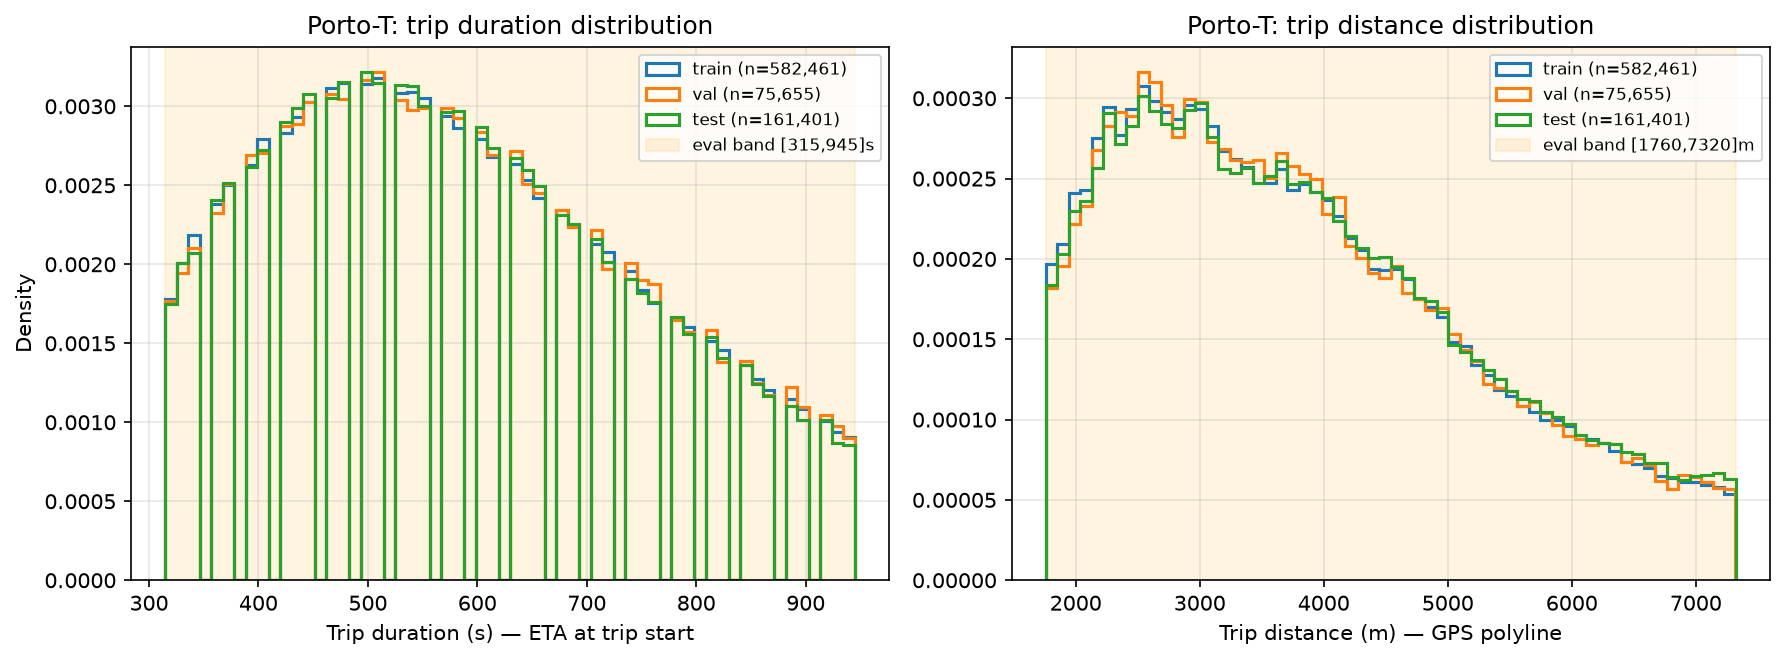
\includegraphics[width=0.95\linewidth]{porto_t_trip_duration_distance_distributions.png}
    \caption{Porto-T trip duration and GPS-polyline distance distributions by chronological split. The split-level curves overlap closely after MetaTTE-style filtering.}\label{fig:porto-t-trip-dist}
\end{figure}

\begin{figure}[!htbp]
    \centering
    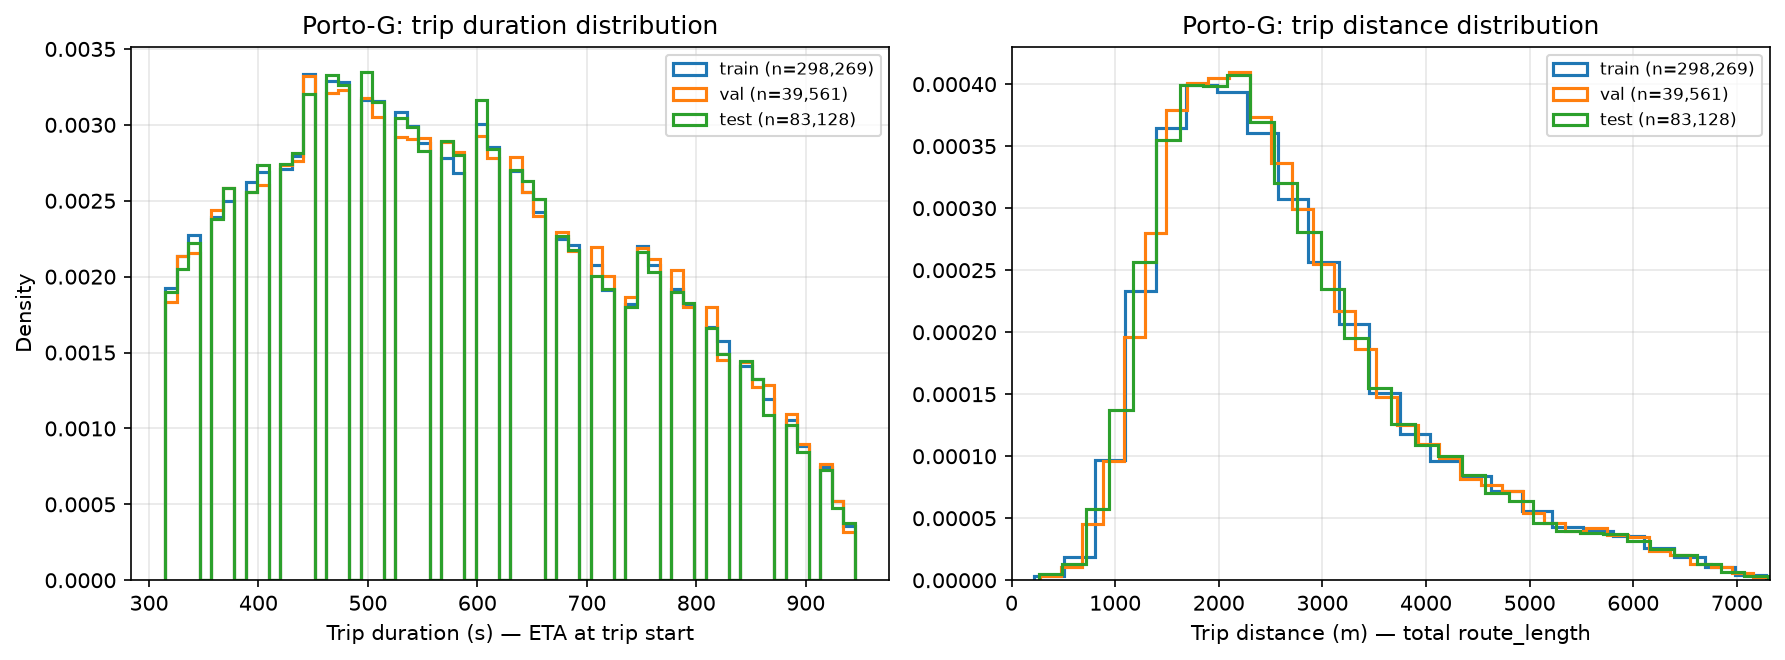
\includegraphics[width=0.95\linewidth]{porto_g_trip_duration_distance_distributions.png}
    \caption{Porto-G trip duration and graph-route distance distributions by chronological split. The split-level curves overlap closely after duration matching.}\label{fig:porto-trip-dist}
\end{figure}

\FloatBarrier

\noindent Figs.~\ref{fig:sumo-trip-dist}--\ref{fig:porto-trip-dist} show trip-duration and trip-distance distributions by chronological split. The train, validation, and test curves overlap closely in all three datasets, supporting the split choice without visible distributional drift. In Fig.~\ref{fig:sumo-trip-dist}, the duration axis is capped at 6{,}000\,s for readability and the dashed vertical line marks the p95 cutoff at 2{,}587\,s. We report SUMO results in both the shared protocol range and the broader p95-filtered population defined in Sect.~\ref{sec:porto-conversion}; even after p95 filtering, SUMO remains broader than the Porto datasets and has a bimodal distance profile, consistent with distinct intra-zone and inter-zone trip populations. Fig.~\ref{fig:porto-g-vs-t} separately compares the Porto-T and Porto-G populations and their different distance definitions.

\begin{figure}[t]
    \centering
    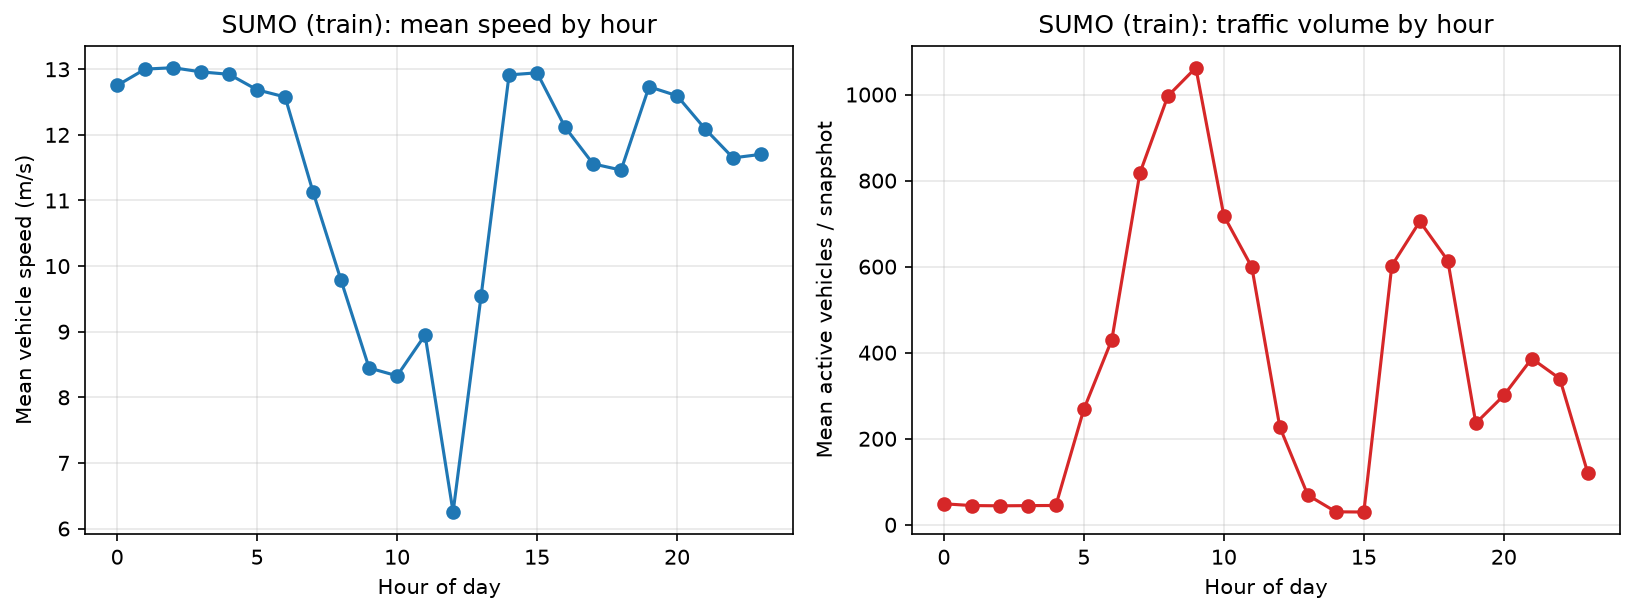
\includegraphics[width=0.95\linewidth]{sumo_speed_volume_by_hour.png}
    \caption{SUMO mean vehicle speed and traffic volume by hour of day (train split). Speed dips and volume peaks coincide at the morning ($\sim$8--9h) and evening ($\sim$17h) rush hours, with a secondary midday volume dip and speed recovery.}\label{fig:sumo-hourly}
\end{figure}

\begin{figure}[t]
    \centering
    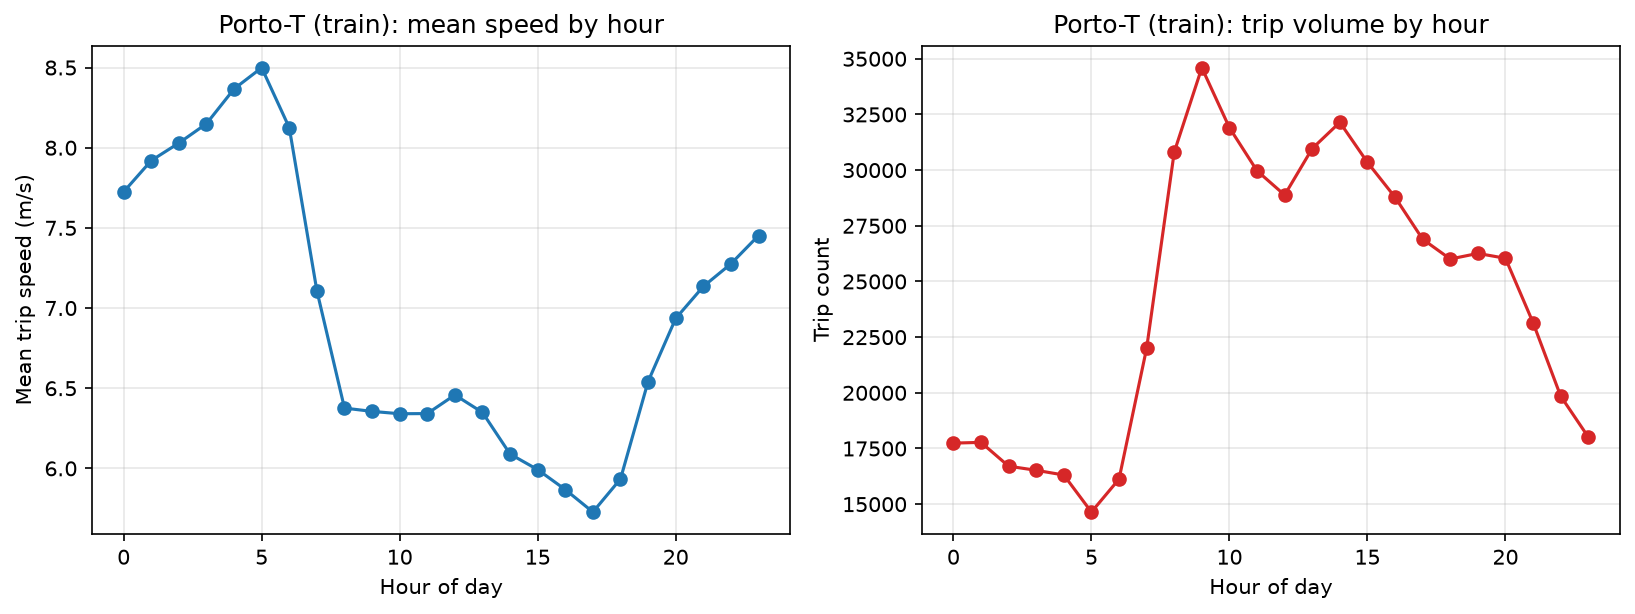
\includegraphics[width=0.95\linewidth]{porto_t_speed_volume_by_hour.png}
    \caption{Porto-T mean trip speed and trip volume by hour of day (train split). Trip volume rises sharply in the morning and remains active through the day, while mean trip speed varies more mildly.}\label{fig:porto-t-hourly}
\end{figure}

\begin{figure}[t]
    \centering
    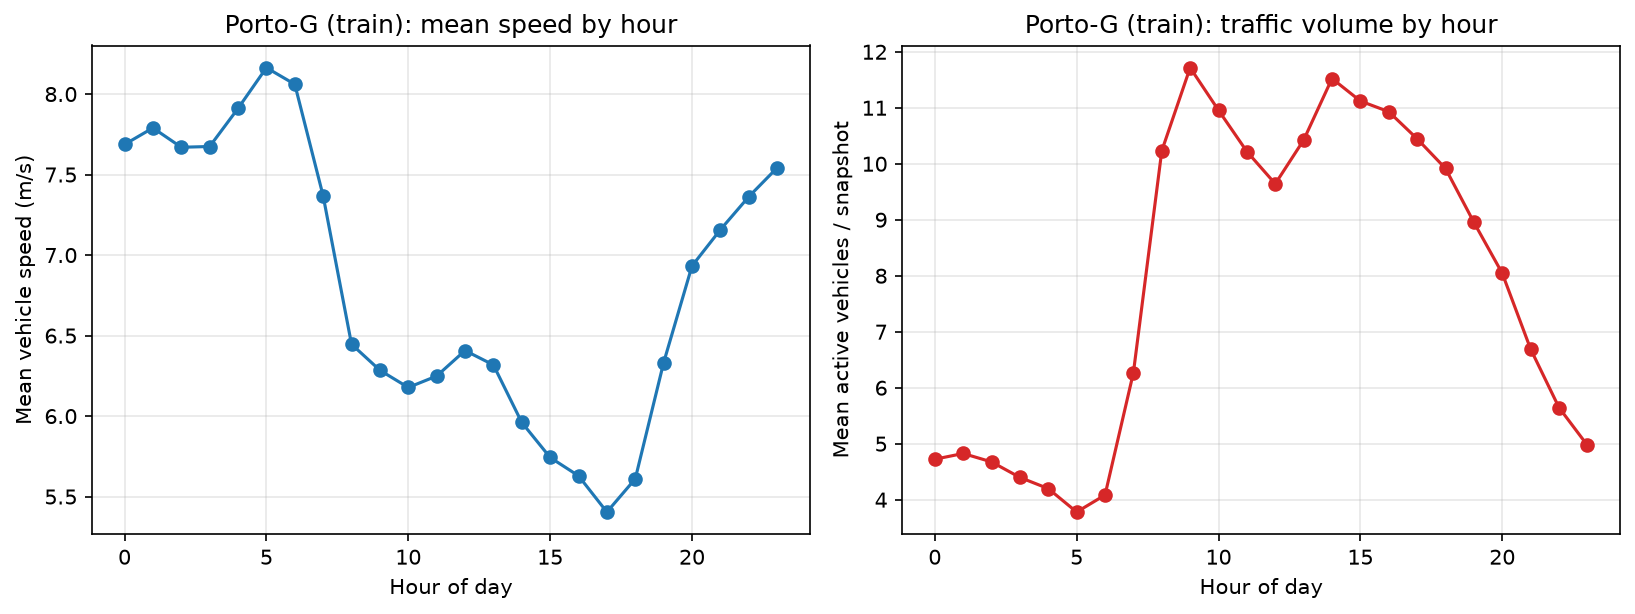
\includegraphics[width=0.95\linewidth]{porto_g_speed_volume_by_hour.png}
    \caption{Porto-G mean vehicle speed and traffic volume by hour of day (train split). The same diurnal pattern recurs at a much smaller scale (single-digit to low-teens active vehicles), with a sharper morning ramp-up and no distinct midday dip.}\label{fig:porto-hourly}
\end{figure}

The hourly profiles in Figs.~\ref{fig:sumo-hourly}--\ref{fig:porto-hourly} show the expected diurnal pattern: traffic volume rises during commuting hours while speed tends to fall. SUMO's profile reflects its scripted peak periods, while Porto-T and Porto-G show taxi-demand patterns at trip and graph-snapshot levels respectively.

\textbf{Limitations.} Porto-G captures one taxi fleet in one city and therefore one traffic mix (no buses/trucks, no zone semantics). Sect.~\ref{sec6} discusses what this scope does and does not support.

\subsection{Evaluation Protocol}\label{sec:eval-protocol}
For SUMO and Porto-G, graph windows are built with $H{=}30$ snapshots (15 minutes) and stride 10; the first $H{-}1$ snapshots of each split are discarded so that no window crosses a split boundary. Porto-T is trip-level and is evaluated directly at the trajectory level.

Protocol-range evaluation uses one prediction per trip start so that graph-based models are compared against trajectory-based baselines on the same unit of prediction: one ETA per trajectory. Porto-G and Porto-T fall within the $[315,945]$\,s protocol range by construction. SUMO is reported in two views: the shared protocol range, and the broader p95-filtered population obtained by retaining vehicles whose trip-start duration is at most 2{,}587\,s as described in Sect.~\ref{sec:porto-conversion}. P95 SUMO tables are then evaluated on the retained vehicles' labeled test rows after applying the $H{=}30$ split-boundary rule.

Training uses the normalized log target defined in Sect.~\ref{sec:loss}. For each dataset and variant, model selection uses the lowest \emph{validation} MAE per seed, with validation reserved exclusively for early stopping and checkpoint selection. All headline numbers are computed on the held-out \emph{test} split: for variants A3--A6, we report the mean $\pm$ std across three seeds (42, 43, 44), while A1 and A2 are reported for seed 42 only. Seed variability is shown for MAE and RMSE, the primary scale-preserving metrics; MAPE is computed directly from predictions and labels but reported as a point estimate because it is secondary and less stable for small ETA denominators.

\subsection{Ablation Variants}\label{sec:ablation-variants}
We compare six code-defined variants (shared encoder and training protocol) on \emph{both} SUMO and Porto-G. Table~\ref{tab:ablation_variants} summarizes the variants and which components are enabled:
\begin{itemize}
    \item \texttt{base\_graph}: static road graph only, no dynamic edges, no temporal, no route features.
    \item \texttt{dynamic\_graph}: adds dynamic edges (junction$\to$vehicle, vehicle$\to$vehicle, vehicle$\to$junction), no temporal, no route features.
    \item \texttt{route\_aware\_graph}: adds route features/encoder and dynamic edges, no temporal.
    \item \texttt{temporal\_base}: temporal context from static-road edges only for the first $H{-}1$ snapshots, no route features, spatial encoder uses only static edges.
    \item \texttt{temporal\_dynamic}: temporal context from the first $H{-}1$ snapshots is aggregated over static-road edges, spatial encoder uses dynamic edges, no route features.
    \item \texttt{temporal\_route\_aware}: full model with dynamic edges, route features/encoder, and temporal context aggregated from static-road edges for the first $H{-}1$ snapshots.
\end{itemize}

\begin{table}[t]
    \centering
    \caption{Ablation variants and enabled components. Temporal uses a GRU over static-road edge sequences for the first $H{-}1$ snapshots. Each variant is trained and evaluated independently on SUMO and on Porto-G.}
    \label{tab:ablation_variants}
    \begin{tabular}{@{}lccc@{}}
        \toprule
        \textbf{Variant} & \textbf{Dyn. Edges} & \textbf{Route Feat.} & \textbf{Temporal} \\
        \midrule
        base\_graph              & --- & --- & --- \\
        dynamic\_graph           & $\checkmark$ & --- & --- \\
        route\_aware\_graph      & $\checkmark$ & $\checkmark$ & --- \\
        temporal\_base           & --- & --- & $\checkmark$ \\
        temporal\_dynamic        & $\checkmark$ & --- & $\checkmark$ \\
        temporal\_route\_aware    & $\checkmark$ & $\checkmark$ & $\checkmark$ \\
        \bottomrule
    \end{tabular}
\end{table}

\subsection{External Baselines}\label{sec:baselines}
To address the concern that comparisons rely mainly on internal ablations and a single average-time baseline, we retrain and evaluate a ladder of external reference methods on Porto-T (trip-level trajectory input) or Porto-G (graph snapshot input), aligning chronological splits, duration range, label definition, and metrics as defined in Sect.~\ref{sec:eval-protocol} and Sect.~\ref{sec:porto-dataset}:
\begin{itemize}
    \item \textbf{AVG}: historical OD-and-hour average travel time, falling back to coarser OD and global averages when a bucket is unseen (MetaTTE-style). Evaluated on Porto-T and SUMO.
    \item \textbf{Linear Regression (LR)}: ridge-regularized linear model over the same trip-geometry features as GBM. Included as a linear ceiling for the tabular feature set and evaluated on Porto-T and SUMO.
    \item \textbf{GBM}: gradient-boosted trees (LightGBM) over trip- and route-geometry features (origin/destination coordinates, polyline or route distance, OD distance, bearing, hour-of-day, day-of-week). Evaluated on Porto-T and SUMO.
    \item \textbf{TEMP}: MetaTTE-style historical segment-speed baseline. Each Porto-T trajectory is split into consecutive GPS segments, and segment travel time is estimated from training-set segment speeds in the same spatial cell and hour-of-day bucket, with cell-only and global-speed fallbacks.
    \item \textbf{Route-sum}: sum of per-edge remaining travel times along \texttt{vehicle\_route\_left}, using per-edge historical average speeds from the training split. Evaluated on Porto-G and SUMO.
    \item \textbf{WDR} (Wide-and-Deep Regression): a wide-and-deep neural model combining a linear component (trip metadata features) with a deep component (learned embeddings) for trip-level ETA prediction. Evaluated on Porto-T.
    \item \textbf{STNN} (Spatio-Temporal Neural Network): a recurrent sequence encoder operating on trip GPS coordinate sequences with spatial and temporal features. Evaluated on Porto-T.
    \item \textbf{DeepTTE}~\cite{deepTTE2018}: our reimplementation of the deep spatial-temporal network for ETA from raw GPS traces, trained on Porto-T with the same calendar split as the graph model.
    \item \textbf{MetaTTE}~\cite{wang2022metatte}: our reimplementation, trained under the same protocol as DeepTTE on Porto-T.
    \item \textbf{DCRNN}~\cite{dcrnn2018}: diffusion convolutional recurrent neural network adapted to the road-edge line graph, predicting per-vehicle ETA from the same $H{=}30$ snapshot window and evaluated on the same graph-native protocol.
\end{itemize}
DeepTTE, MetaTTE, TEMP, WDR, and STNN use trip-level Porto-T inputs. AVG, LR, and GBM use trip/geometry tables derived from Porto-T or SUMO; Route-sum, DCRNN, and DSTRA-GNN use graph snapshots on Porto-G or SUMO. SUMO is used for both controlled DSTRA-GNN ablations and a compact p95 external-baseline comparison.

\subsection{Evaluation Metrics}
We report Mean Absolute Error (MAE) and Root Mean Squared Error (RMSE) in seconds, and Mean Absolute Percentage Error (MAPE), computed directly from stored predictions and ground-truth labels (not estimated).

% ===== END sections/experiments.tex =====



% ===== BEGIN sections/results.tex =====
\section{Results and Analysis}\label{sec5}

Unless stated otherwise, all numbers reported below follow the evaluation protocol defined in Sect.~\ref{sec:eval-protocol}.

\subsection{Ablation Study}\label{sec5:ablation}

Tables~\ref{tab:ablation_porto} and~\ref{tab:ablation_sumo} report per-variant test-set metrics in the shared protocol range, which supports direct comparison between Porto-G and SUMO. Table~\ref{tab:ablation_sumo_p95} then evaluates the same SUMO variants on the broader p95-filtered SUMO population defined in Sect.~\ref{sec:porto-conversion}. Each row isolates a specific combination of dynamic edges, route features, and GRU temporal context, with component toggles defined in Sect.~\ref{sec:ablation-variants}.

\begin{table}[t]
    \centering
    \caption{Ablation study on Porto-G (test set, evaluation protocol, $n{=}106{,}636$ trips). A3--A6 report mean $\pm$ std across seeds 42/43/44. A1--A2 use seed 42 only. \textbf{Bold} = best per column.}
    \label{tab:ablation_porto}
    {\footnotesize\setlength{\tabcolsep}{4pt}%
    \begin{tabular}{@{}llccc@{}}
        \toprule
        \textbf{Variant} & \textbf{Components} & \textbf{MAE (s)} & \textbf{RMSE (s)} & \textbf{MAPE (\%)} \\
        \midrule
        A1 \texttt{base\_graph}            & Static only         & 93.29 & 122.04 & 17.28 \\
        A2 \texttt{dynamic\_graph}         & +Dyn.\ edges        & 91.76 & 120.63 & 16.88 \\
        A3 \texttt{route\_aware\_graph}    & +Route+Dyn.\        & 74.81 $\pm$ 0.52 & 100.30 $\pm$ 0.88 & 13.96 \\
        A4 \texttt{temporal\_base}         & +Temp.\ (GRU)       & 90.00 $\pm$ 0.66 & 118.67 $\pm$ 1.01 & 17.05 \\
        A5 \texttt{temporal\_dynamic}      & +Temp.+Dyn.\        & 87.99 $\pm$ 0.61 & 107.83 $\pm$ 0.94 & 16.76 \\
        A6 \texttt{temporal\_route\_aware} & Full model (GRU)    & \textbf{68.05 $\pm$ 0.48} & \textbf{90.01 $\pm$ 0.86} & \textbf{13.20} \\
        \bottomrule
    \end{tabular}}%
\end{table}

\begin{table}[t]
    \centering
    \caption{Ablation study on SUMO (test set, protocol range, $n{=}103{,}144$ trips). A3--A6 report mean $\pm$ std across seeds 42/43/44. A1--A2 use seed 42 only. \textbf{Bold} = best per column.}
    \label{tab:ablation_sumo}
    {\footnotesize\setlength{\tabcolsep}{4pt}%
    \begin{tabular}{@{}llccc@{}}
        \toprule
        \textbf{Variant} & \textbf{Components} & \textbf{MAE (s)} & \textbf{RMSE (s)} & \textbf{MAPE (\%)} \\
        \midrule
        A1 \texttt{base\_graph}            & Static only         & 80.10 & 211.86 & 12.03 \\
        A2 \texttt{dynamic\_graph}         & +Dyn.\ edges        & 74.96 & 135.63 & 11.59 \\
        A3 \texttt{route\_aware\_graph}    & +Route+Dyn.\        & 66.81 $\pm$ 0.64 & 110.23 $\pm$ 0.93 & 10.06 \\
        A4 \texttt{temporal\_base}         & +Temp.\ (GRU)       & 76.29 $\pm$ 0.73 & 121.26 $\pm$ 1.08 & 12.05 \\
        A5 \texttt{temporal\_dynamic}      & +Temp.+Dyn.\        & 64.08 $\pm$ 0.66 & 97.38 $\pm$ 1.01 & 9.76 \\
        A6 \texttt{temporal\_route\_aware} & Full model (GRU)    & \textbf{54.75 $\pm$ 0.71} & \textbf{82.72 $\pm$ 0.96} & \textbf{8.33} \\
        \bottomrule
    \end{tabular}}%
\end{table}

\begin{table}[t]
    \centering
    \caption{Ablation study on SUMO (test set, p95-filtered population retaining vehicles with trip-start duration $\leq 2{,}587$\,s). Metrics are computed over retained vehicles' labeled test rows after the $H{=}30$ window boundary. A3--A6 report mean $\pm$ std across seeds 42/43/44. A1--A2 use seed 42 only. \textbf{Bold} = best per column.}
    \label{tab:ablation_sumo_p95}
    {\footnotesize\setlength{\tabcolsep}{4pt}%
    \begin{tabular}{@{}llccc@{}}
        \toprule
        \textbf{Variant} & \textbf{Components} & \textbf{MAE (s)} & \textbf{RMSE (s)} & \textbf{MAPE (\%)} \\
        \midrule
        A1 \texttt{base\_graph}            & Static only         & 78.33 & 235.56 & 25.13 \\
        A2 \texttt{dynamic\_graph}         & +Dyn.\ edges        & 77.56 & 244.34 & 23.54 \\
        A3 \texttt{route\_aware\_graph}    & +Route+Dyn.\        & 76.22 $\pm$ 1.42 & 218.98 $\pm$ 2.01 & 22.34 \\
        A4 \texttt{temporal\_base}         & +Temp.\ (GRU)       & 80.38 $\pm$ 1.23 & 232.16 $\pm$ 2.12 & 24.35 \\
        A5 \texttt{temporal\_dynamic}      & +Temp.+Dyn.\        & 75.81 $\pm$ 1.82 & 219.22 $\pm$ 2.19 & 22.22 \\
        A6 \texttt{temporal\_route\_aware} & Full model (GRU)    & \textbf{72.44 $\pm$ 1.31} & \textbf{214.50 $\pm$ 2.92} & \textbf{19.71} \\
        \bottomrule
    \end{tabular}}%
\end{table}

\begin{table}[t]
    \centering
    \caption{External baseline comparison on SUMO (test set, p95-filtered population retaining vehicles with trip-start duration $\leq 2{,}587$\,s). Classical and graph-native baselines are evaluated over the same retained labeled test rows as Table~\ref{tab:ablation_sumo_p95}. \textbf{Bold} = best per column.}
    \label{tab:baselines_sumo_p95}
    {\footnotesize\setlength{\tabcolsep}{4pt}%
    \begin{tabular}{@{}llccc@{}}
        \toprule
        \textbf{Model} & \textbf{Type} & \textbf{MAE (s)} & \textbf{RMSE (s)} & \textbf{MAPE (\%)} \\
        \midrule
        AVG (OD-hour)       & Non-parametric   & 174.34 & 471.50 & 78.68 \\
        Linear Regression   & Statistical      & 654.78 & 819.03 & 338.18 \\
        GBM (LightGBM)      & Gradient boosting & 276.41 & 419.62 & 64.65 \\
        Route-sum           & Graph heuristic  & 481.64 & 620.92 & 86.41 \\
        DCRNN~\cite{dcrnn2018} & Graph neural net & 228.44 & 438.38 & 53.91 \\
        A6 (full model)     & DSTRA-GNN        & \textbf{72.44} & \textbf{214.50} & \textbf{19.71} \\
        \bottomrule
    \end{tabular}}%
\end{table}

\textbf{Route intent is the dominant non-temporal factor on both domains.} Adding explicit route features on top of dynamic edges (A2$\to$A3) delivers the largest single gain among the non-temporal variants under the protocol-range evaluation: Porto-G MAE drops 18.5\% (91.76\,s to 74.81\,s) and SUMO MAE drops 10.9\% (74.96\,s to 66.81\,s). Dynamic interaction edges alone (A1$\to$A2) help less and to a different degree on each domain: only 1.6\% on Porto-G's sparse taxi fleet ($\sim$10--15 active vehicles per snapshot) versus 6.4\% on SUMO's denser traffic mix ($\sim$280 active vehicles per snapshot). GRU temporal aggregation on top of the full route-aware representation (A3$\to$A6) yields a further substantial reduction on both domains: 9.0\% on Porto-G and 18.1\% on SUMO. On the broader p95-filtered SUMO population, the same ordering remains: the full model achieves the lowest MAE at 72.44\,s, compared with 75.81\,s for A5 and 76.22\,s for A3. Table~\ref{tab:baselines_sumo_p95} further shows that this result is not only an internal ablation win: the full model also outperforms AVG, LR, GBM, Route-sum, and DCRNN on the retained SUMO test population.

\begin{figure}[t]
    \centering
    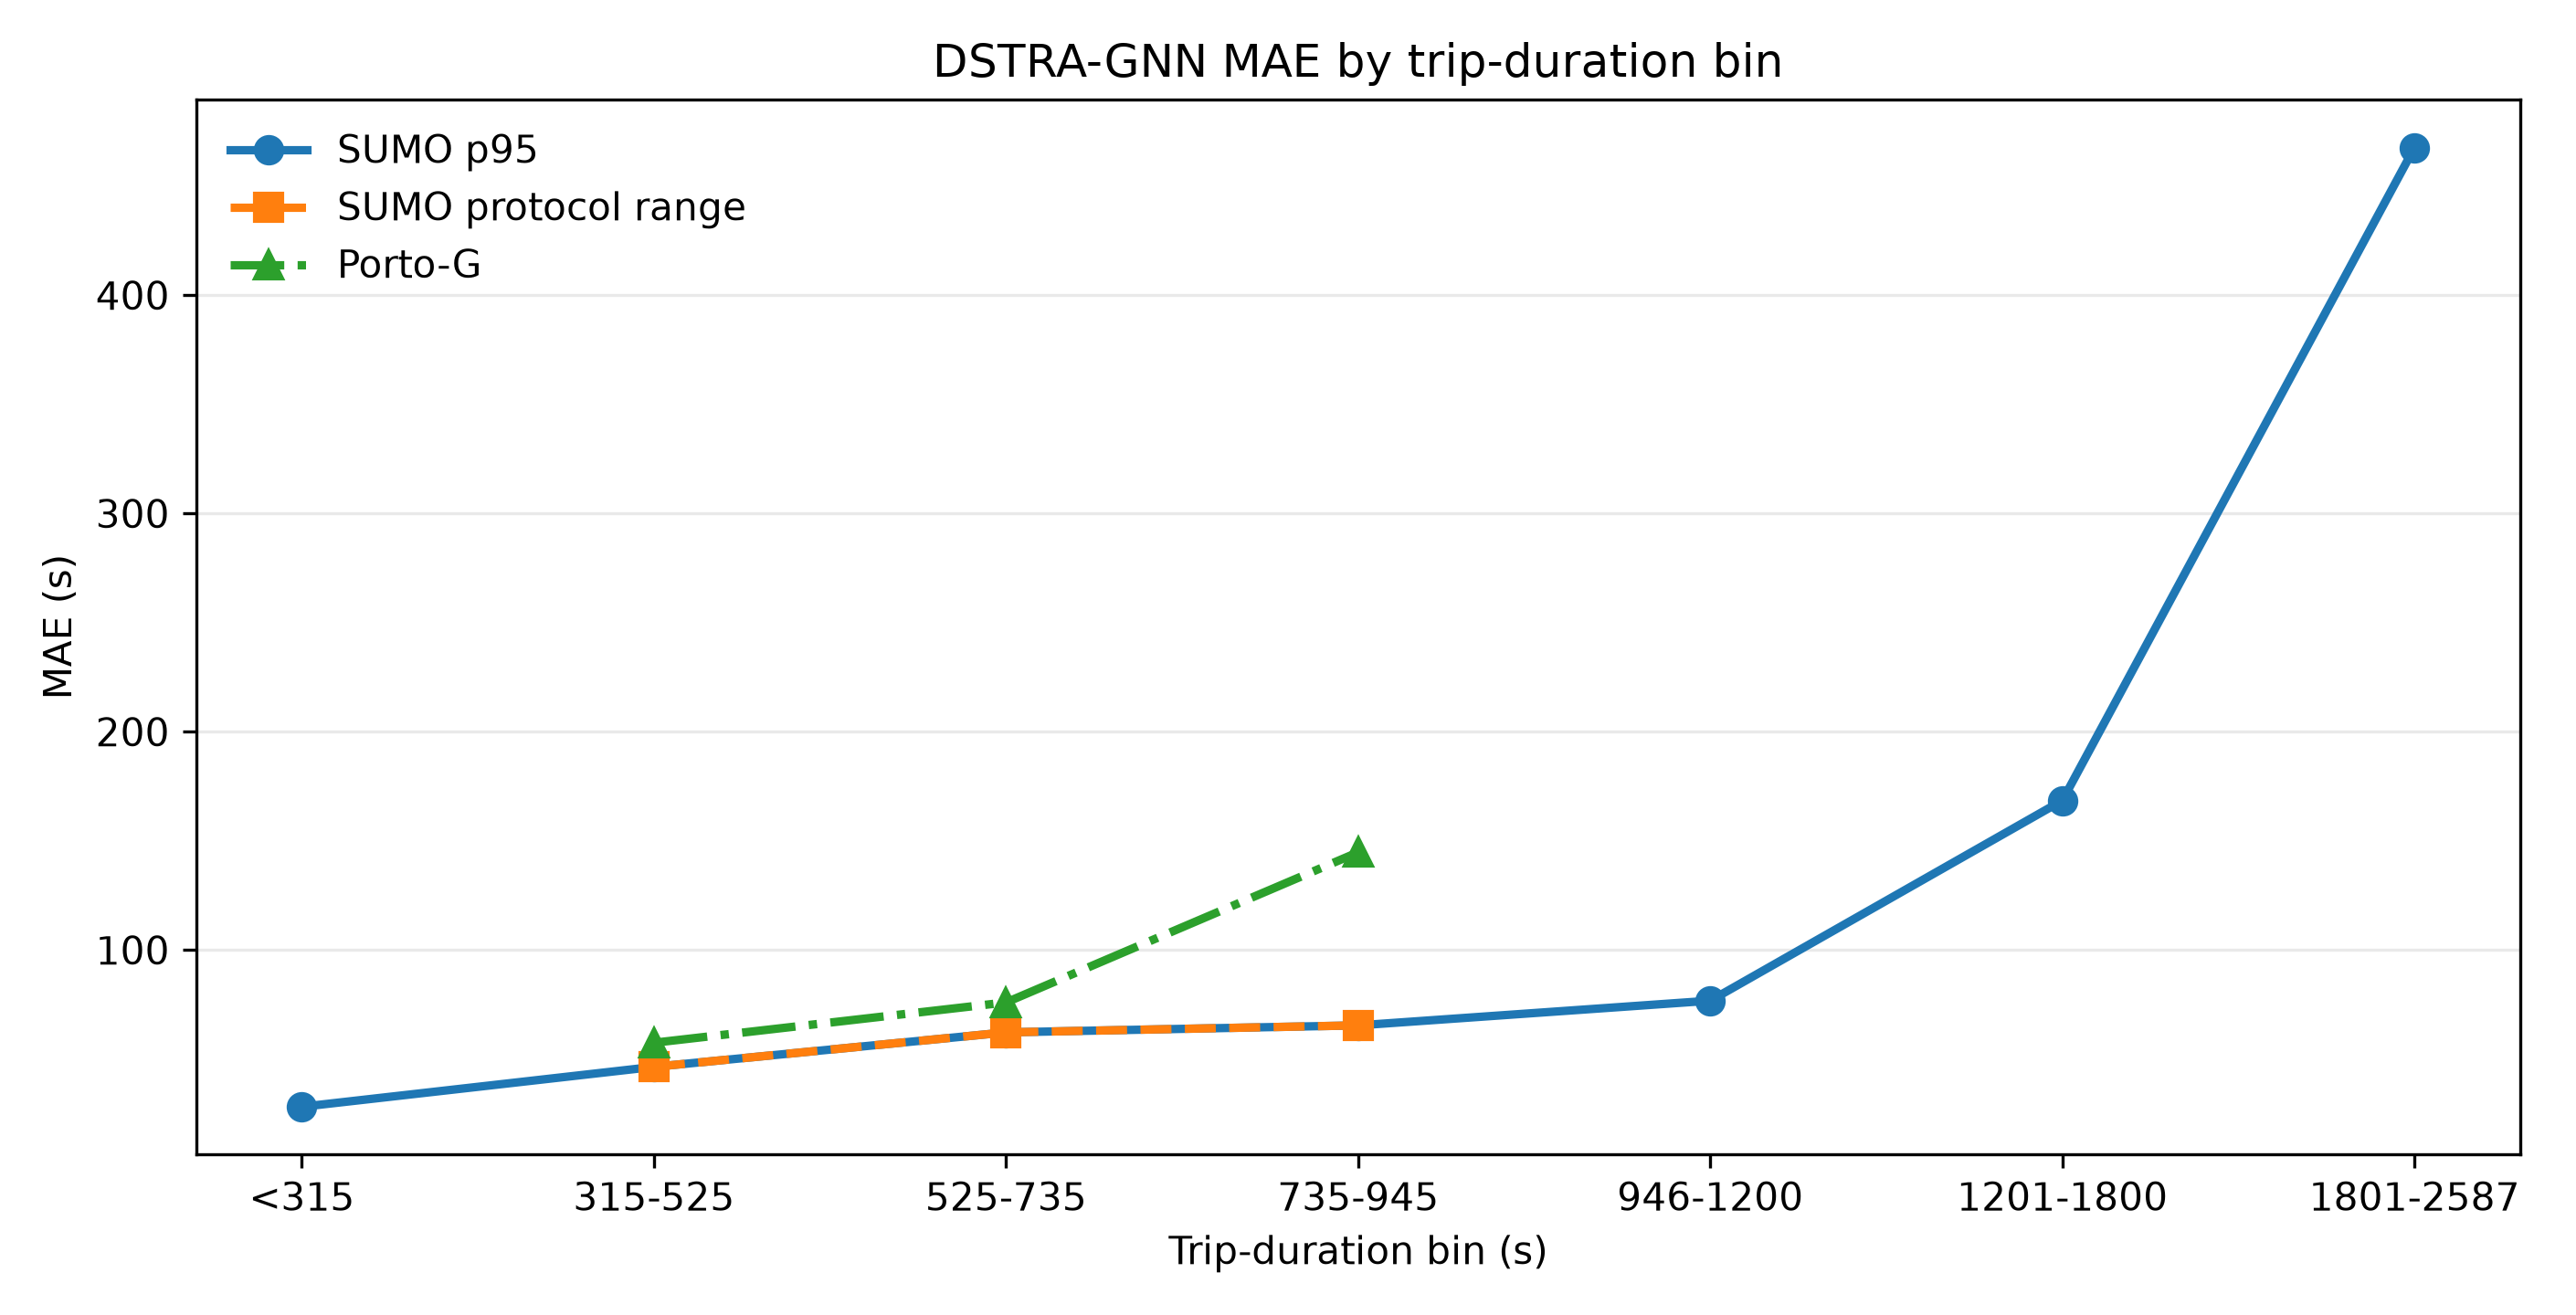
\includegraphics[width=0.88\linewidth]{dstra_trip_duration_bin_mae.png}
    \caption{DSTRA-GNN A6 trip-start MAE by duration bin on SUMO p95, SUMO protocol range, and Porto-G. Bins are $<315$, $315$--$525$, $525$--$735$, $735$--$945$, $946$--$1200$, $1201$--$1800$, and $1801$--$2587$\,s; the three interior bins split the shared $[315,945]$\,s protocol band.}
    \label{fig:dstra-duration-bin-mae}
\end{figure}

Fig.~\ref{fig:dstra-duration-bin-mae} shows that error increases with trip duration across both graph domains. The SUMO p95 curve extends beyond the shared protocol range up to the 2{,}587\,s cutoff, while the SUMO protocol-range and Porto-G curves occupy the common $[315,945]$\,s comparison band.

\subsection{Porto Baseline Comparison}\label{sec5:baselines}

Table~\ref{tab:baselines_porto} compares DSTRA-GNN against a ladder of external baselines on Porto using the protocol defined in Sect.~\ref{sec:eval-protocol}. Trajectory baselines (AVG, LR, GBM, TEMP, DeepTTE, MetaTTE, WDR, STNN) use Porto-T, whose test split is itself restricted to the $[315,945]$\,s protocol range. Graph-native baselines (Route-sum, DCRNN, DSTRA-GNN) use Porto-G, the duration-matched graph-converted subset of the same Porto source. Because the input modality and exact trip populations differ, this is a cross-representation comparison rather than a paired trip-identical test; we therefore report all models on the same metrics and label the input format explicitly in the caption.

\begin{table}[t]
    \centering
    \caption{Baseline comparison on Porto (test set, evaluation protocol). \emph{Porto-T}: trip-level trajectory input. \emph{Porto-G}: duration-matched graph snapshot input converted from Porto-T trajectories. All use the same chronological calendar split (test: 2014-05-01 to 2014-07-01), but Porto-T and Porto-G are not exact trip-identical test populations. DSTRA-GNN reports mean across seeds 42/43/44 ($\pm$ std for MAE/RMSE: 68.05$\pm$0.48 / 90.01$\pm$0.86). \textbf{Bold} = best per column.}
    \label{tab:baselines_porto}
    \begin{tabular}{@{}llcccr@{}}
        \toprule
        \textbf{Model} & \textbf{Input} & \textbf{MAE (s)} & \textbf{RMSE (s)} & \textbf{MAPE (\%)} & \textbf{$n$} \\
        \midrule
        \multicolumn{6}{@{}l}{\textit{Non-parametric / statistical}} \\
        AVG (OD-hour)       & Porto-T & 113.29 & 142.54 & 20.83 & 161{,}401 \\
        Linear Regression   & Porto-T & 107.58 & 133.89 & 19.67 & 161{,}401 \\
        GBM (LightGBM)      & Porto-T &  86.41 & 113.21 & 15.00 & 161{,}401 \\
        TEMP                & Porto-T & 113.34 & 148.02 & 19.87 & 161{,}401 \\
        Route-sum           & Porto-G & 226.15 & 260.42 & 41.02 & 106{,}647 \\
        \midrule
        \multicolumn{6}{@{}l}{\textit{Deep learning (trajectory-native)}} \\
        DeepTTE~\cite{deepTTE2018}     & Porto-T &  68.59 &  90.68 & \textbf{12.13} & 161{,}400 \\
        MetaTTE~\cite{wang2022metatte} & Porto-T &  69.46 &  91.74 & 12.34 & 161{,}400 \\
        WDR                 & Porto-T &  72.11 &  94.60 & 12.81 & 161{,}400 \\
        STNN                & Porto-T &  74.15 &  97.27 & 13.05 & 161{,}400 \\
        \midrule
        \multicolumn{6}{@{}l}{\textit{Graph-native spatio-temporal}} \\
        DCRNN~\cite{dcrnn2018}         & Porto-G & 131.32 & 172.82 & 28.95 & 106{,}647 \\
        \midrule
        \multicolumn{6}{@{}l}{\textit{DSTRA-GNN (this work)}} \\
        A6 (full model)     & Porto-G & \textbf{68.05} & \textbf{90.01} & 13.20 & 106{,}636 \\
        \bottomrule
    \end{tabular}
\end{table}

\textbf{Classical and tabular baselines.} On Porto, GBM (86.41\,s) is the strongest tabular baseline, comfortably outperforming AVG (113.29\,s), LR (107.58\,s), and the TEMP historical segment-speed baseline (113.34\,s), while Route-sum (226.15\,s) is the weakest despite having access to explicit route geometry -- likely because per-edge historical speeds on Porto-G are estimated from sparse taxi observations and degrade when any edge is rarely traversed.

\textbf{Deep sequence baselines on Porto.} DeepTTE (68.59\,s) and MetaTTE (69.46\,s) are the strongest non-graph baselines, followed closely by WDR (72.11\,s) and STNN (74.15\,s). All four deep trajectory models are trained on Porto-T with the same chronological split and are reimplemented here to align the calendar split, label range, and metrics with the graph evaluation. Their advantage over GBM (86.41\,s) shows that learning from the spatial sequence of GPS positions adds value beyond hand-crafted trip features.

\textbf{DCRNN on Porto-G.} DCRNN adapted to the Porto-G road-edge line graph (131.32\,s) performs worse than the tabular and sequence baselines but better than the simple Route-sum heuristic. We attribute this gap to the representation mismatch: DCRNN is designed for densely observed road networks with regular link-level signals, whereas Porto-G is a sparse, single-fleet snapshot dataset with only a small number of active vehicles per snapshot.

\textbf{DSTRA-GNN relative to the baseline ladder.} On Porto, the full model (A6) falls in the same accuracy band as the strongest trajectory-native deep baselines: 68.05\,s MAE and 90.01\,s RMSE on Porto-G, compared with DeepTTE at 68.59\,s/90.68\,s and MetaTTE at 69.46\,s/91.74\,s on Porto-T. DeepTTE retains a marginally lower MAPE (12.13\% vs.\ 13.20\%), so the comparison should be read as close positioning among high-accuracy models rather than a decisive separation. On SUMO, where trajectory-native DeepTTE/MetaTTE-style inputs are not available, the ablation tables show that DSTRA-GNN's full route-aware temporal configuration is the most accurate graph variant in both reported views, and Table~\ref{tab:baselines_sumo_p95} shows it also outperforms the applicable classical and graph-native baselines on the retained p95 population. These results situate DSTRA-GNN among the more accurate models while evaluating a graph-native, route-aware representation rather than a trajectory-native sequence encoder.

% ===== END sections/results.tex =====



% ===== BEGIN sections/discussion.tex =====
\section{Discussion}\label{sec6}

\textbf{Route intent dominates in both domains.} Under the shared protocol range, adding explicit route features on top of dynamic edges (A2$\to$A3) gives the largest single non-temporal gain: SUMO MAE falls from 74.96\,s to 66.81\,s (10.9\%), and Porto-G falls from 91.76\,s to 74.81\,s (18.5\%). This pattern also remains visible on the broader p95-filtered SUMO population, where route-aware variants remain stronger than their non-route counterparts. The consistency across controlled simulation and real taxi trips supports the central claim that exposing a vehicle's remaining planned path resolves much of the destination/route ambiguity that static or dynamic-edge-only representations must otherwise infer implicitly. The ablation grid isolates the incremental value of route features when added to the dynamic graph (A2$\to$A3 and A5$\to$A6), but it does not include a route-only static-graph variant; we therefore interpret these gains as evidence for explicit route intent within the tested dynamic-graph family rather than as a complete factorial decomposition of route and dynamic-edge effects.

Route information has different provenance across domains: SUMO uses pre-planned shortest paths, whereas Porto-G uses map-matched driven paths from observed taxi traces. We therefore interpret cross-domain consistency as evidence that exposing remaining path structure is useful under both route-generation regimes, not that both datasets share an identical route-planning assumption.

\textbf{Dynamic edges are useful, but secondary to route intent.} Adding dynamic edges \emph{without} route features (A1$\to$A2) helps on both domains under the protocol-range evaluation, but to different degrees: 1.6\% on Porto-G's sparse taxi fleet ($\sim$10--15 active vehicles per snapshot, 93.29\,s$\to$91.76\,s) versus 6.4\% on SUMO's denser traffic mix ($\sim$280 active vehicles per snapshot, 80.10\,s$\to$74.96\,s). This is the opposite of a density-dilution hypothesis, under which SUMO's much larger number of short-lived junction$\to$vehicle and vehicle$\to$vehicle edges would be expected to add noise rather than signal. Instead, SUMO's denser interaction graph appears to carry usable local context. Route features remain the larger lever in absolute terms on both domains, but dynamic edges are not merely noise. A systematic density-stratified study of dynamic-edge attention (e.g., across SUMO's lower-traffic hours) is left to future work.

\textbf{Temporal context complements rather than substitutes for spatial structure.} GRU-based temporal aggregation over the static road-edge sequence, introduced in Sect.~\ref{sec3}, helps on both domains, and its marginal contribution grows with how much spatial structure is already present in the representation. Added alone on top of the static graph (A1$\to$A4), temporal context reduces MAE by 3.5\% on Porto-G and 4.8\% on SUMO. Added on top of the full dynamic+route representation (A3$\to$A6), the same temporal module instead reduces MAE by 9.0\% on Porto-G and 18.1\% on SUMO. We interpret this as evidence that the GRU's recurrent summary of the last 29 static-edge snapshots is most useful once the model also has route intent and local interaction context to combine it with, rather than as a substitute for either. The effect is larger on SUMO, where temporal congestion buildup is more pronounced, as Sect.~\ref{sec4} shows. A systematic density-stratified analysis of when temporal context helps most is left to future work.

\textbf{Positioning against the literature.} As discussed in Sect.~\ref{sec2}, headline numbers reported for related systems (DuETA, DCRNN, DeepTTE, ConSTGAT~\cite{dueta2023,dcrnn2018,deepTTE2018,constgat2020}) are not directly comparable across differing cities, label definitions, and time horizons. Our positioning is therefore empirical: Table~\ref{tab:baselines_porto} compares against baselines retrained under a shared Porto calendar split, duration range, and metric set, while making clear that Porto-G is a duration-matched graph-converted population rather than the exact Porto-T trajectory test set. Although Porto-G and Porto-T originate from the same raw dataset, they constitute different learning tasks and representations: Porto-T operates directly on GPS trajectories, whereas Porto-G requires route reconstruction, graph conversion, and snapshot aggregation. Under this cross-representation comparison, the full model falls in the same accuracy band as DeepTTE and MetaTTE~\cite{wang2022metatte}, to our knowledge the strongest open, trajectory-native baselines published for this task. DSTRA-GNN uses graph snapshots with explicit remaining-route state, whereas DeepTTE and MetaTTE encode trajectory sequences. On SUMO, the ablation tables position the full route-aware temporal model as the strongest evaluated DSTRA-GNN variant under both the shared protocol range and the broader p95-filtered population.

\textbf{Fairness and observability.} Although SUMO is simulation-based, route-aware ETA and dispatch decisions can have distributional effects across the network's zones. Better calibrated ETA estimates can support mobility reliability by reducing missed arrivals, inefficient dispatch, and avoidable rerouting, but the present evaluation measures prediction accuracy rather than downstream emissions, accessibility, or equity outcomes. A natural extension is to report per-zone error breakdowns to check that gains are not concentrated in already-well-served areas (e.g., the urban grid zones) at the expense of the suburban ring or connector zones. Porto-G, lacking zone labels, cannot support this analysis and would need an auxiliary geographic partition if pursued. Separately, several of the dynamic features used here -- \texttt{vehicles\_on\_road\_count}, interaction edges, per-vehicle positions -- presuppose a sensing capability (GPS-equipped fleets or roadside infrastructure reporting vehicle counts/positions in near real time) that SUMO provides for free but that a real deployment would need to justify on privacy/surveillance grounds. Porto-G, being derived from individual taxi GPS traces, illustrates the kind of data such a deployment would require and the associated data-governance considerations.

\textbf{Limitations.} The p95 filter removes SUMO's rare extreme-duration simulator tail, so the broader SUMO results should be read as performance on the retained generated population rather than on every possible simulated artifact. Porto-G covers a single taxi fleet in one city, has no zone semantics, and is a duration-matched converted subset of Porto-T rather than a trip-identical copy of the trajectory benchmark. Because Porto-G uses route reconstruction from observed traces rather than real navigation logs, no route re-planning events are observed. It should be read as evidence that the SUMO-derived representation and gains transfer to real trips, not as a second controlled benchmark at matching scale. Finally, the dynamic-edge and temporal findings above are based on a single real-world domain (Porto-G) at one density regime. Broader claims about density-dependence would benefit from additional real-world cities once suitable open trajectory data becomes available, as discussed further in Sect.~\ref{sec4}.

% ===== END sections/discussion.tex =====



% ===== BEGIN sections/conclusion.tex =====
\section{Conclusion}\label{sec7}

This work introduced DSTRA-GNN, a dynamic spatio-temporal graph neural network for ETA prediction that unifies static road infrastructure, per-vehicle dynamics, and explicit route intent within a Mixture-of-Experts framework. Its central idea is to represent traffic as a vehicle-centered dynamic graph: persistent road edges provide the stable transport topology, while vehicle and interaction edges expose the local state needed for per-vehicle ETA prediction.

We evaluated the model on a large-scale p95-filtered SUMO simulation dataset (four weeks, 80{,}693 snapshots, 798{,}919 retained trips) and on Porto-G, a graph representation of Porto taxi trajectories derived from the ECML-PKDD 2015 dataset. Across six ablation variants, route awareness and GRU-based temporal context provide consistent, compounding gains. Under the shared protocol range, the full model reduces MAE from 93.29\,s to 68.05\,s on Porto-G (27\%) and from 80.10\,s to 54.75\,s on SUMO (32\%). On the broader p95-filtered SUMO population, it remains the strongest evaluated variant at 72.44\,s MAE and outperforms the applicable AVG, LR, GBM, Route-sum, and DCRNN baselines.

On Porto, DSTRA-GNN falls in the same accuracy band as trajectory-native deep baselines such as DeepTTE and MetaTTE, while using a duration-matched graph-native representation with explicit remaining-route state. This cross-representation result supports the paper's main claim: public, route-aware dynamic graph representations can reproduce key advantages of production route-aware ETA systems in an open experimental setting, even though exact trip-identical Porto-T/Porto-G evaluation remains future work.

Future work includes extending the evaluation to additional real-world cities as dense open trajectory datasets become available, investigating density-stratified dynamic-edge ablations, and exploring per-zone fairness analyses to ensure that ETA gains are distributed evenly across urban, suburban, and connector zones. Longer-horizon trips remain an important regime for future work and may benefit from uncertainty-aware prediction heads or route-segment-level auxiliary supervision.

% ===== END sections/conclusion.tex =====


\backmatter


% ===== BEGIN sections/declarations.tex =====
\section*{Declarations}

\subsection*{Funding}
This study was funded by grant number 34836 from the Israeli Ministry of Innovation, Science and Technology (Proposal no. 0007846).

\subsection*{Competing Interests}
The authors declare that they have no competing interests.

\subsection*{Ethics approval and consent to participate}
Not applicable.

\subsection*{Consent for publication}
Not applicable.

\subsection*{Data availability}
Two datasets are used in this study, both publicly available on Kaggle. The SUMO dataset is a simulation-derived dynamic traffic dataset built with the Eclipse SUMO traffic simulator~\cite{SUMO2018} and is available at~\cite{tordjman2026sumokaggle}. It can also be regenerated using the dataset generation tool~\cite{sumo_data_generator}. The Porto-G dataset is derived from the publicly available Porto taxi trajectory data released for the ECML-PKDD 2015 Taxi Trajectory Prediction challenge~\cite{moreira2013porto}, converted to the graph representation described in Sect.~\ref{sec:porto-conversion}, and is available at~\cite{tordjman2026portokaggle}. The conversion pipeline is included with the model code.

\subsection*{Materials availability}
Not applicable.

\subsection*{Code availability}
The code and implementation details are available in the following GitHub repositories: the dataset generation tool~\cite{sumo_data_generator} for generating the simulation-derived dynamic traffic dataset used in this study, and the test environment~\cite{trafficlab} for testing and validating the model implementation. The DSTRA-GNN model, Porto-G conversion pipeline, training scripts, and all retrained external baselines (AVG, LR, GBM, TEMP, Route-sum, WDR, STNN, DeepTTE, MetaTTE, DCRNN) corresponding to the results reported here are available at commit \texttt{a45a089} of the same repository.

\subsection*{Acknowledgements}
The authors would like to thank Ruppin Academic Center, Israel, and the Israeli Ministry of Innovation, Science and Technology (Proposal no. 0007846), for the continuing support in this research, implementation, and presentation.

\subsection*{Author contribution}
All authors contributed to the study conception and design. Material preparation, data collection and analysis were performed by Guy Tordjman and Nadav Voloch. The first draft of the manuscript was written by Guy Tordjman and all authors commented on previous versions of the manuscript. All authors read and approved the final manuscript.

% ===== END sections/declarations.tex =====


\bibliography{references}

\end{document}
